\documentclass[a4j,11pt]{jsarticle}
\usepackage{semi}
\usepackage{breqn}
\usepackage{tabularx}
\usepackage{listings,jlisting}
\usepackage{latexsym}
\usepackage{anyfontsize}
\lstset{
  basicstyle={\ttfamily},
  identifierstyle={\small},
  commentstyle={\smallitshape},
  keywordstyle={\small\bfseries},
  ndkeywordstyle={\small},
  stringstyle={\small\ttfamily},
  frame={tb},
  breaklines=true,
  columns=[l]{fullflexible},
  numbers=left,
  xrightmargin=0zw,
  xleftmargin=3zw,
  numberstyle={\scriptsize},
  stepnumber=1,
  numbersep=1zw,
  lineskip=-0.5ex
}

\newcolumntype{Y}{&gt;{\centering\arraybackslash}X} %中央揃え
 
\makeatletter % プリアンブルで定義開始

% 図番号を"<章節などの番号番号> - <図番号>" へ
\renewcommand{\thefigure}{\thesubsection-\arabic{figure}}
\renewcommand{\thetable}{\thesubsection-\arabic{table}}
% 章が進むごとに図番号をリセットする
\@addtoreset{figure}{subsection}
\@addtoreset{table}{section}
\renewcommand{\theequation}{% 式番号の付け方
	\thesection.\arabic{equation}}
	\@addtoreset{equation}{section}
\makeatother % プリアンブルで定義終了

\renewcommand{\headfont}{\bfseries} %章タイトルなどを明朝体にする

\makeindex
\begin{document}
\definecolor{cellcolor}{rgb}{ 1, .90, .90}
\definecolor{rowcolor}{rgb}{.85, .85, 1}
\setcounter{tocdepth}{3}
\thispagestyle{empty}
\clearpage
\addtocounter{page}{-1}
\begin{center}

\huge
2019年度 卒業論文\\[60pt]
\HUGE
逆畳込みとケプストラム法を\\
組み合わせることによる\\
残響除去手法の提案\\[65pt]
\huge
指導教員 須田 宇宙 准教授\\[40pt]
千葉工業大学 情報ネットワーク学科\\[10pt]
須田研究室\\[40pt]
1632038 \hspace{70pt} 岡田 秀\\[110pt]
\end{center}
\begin{flushright} 
\huge

\textcolor{white}{文字}

\textcolor{white}{文字}

提出日 2020年1月30日
\end{flushright}
\newpage
\thispagestyle{empty}
\clearpage
\addtocounter{page}{-1}
\large
% 目次
\tableofcontents
\thispagestyle{empty}
\clearpage
\addtocounter{page}{-1}
\newpage
%表目次
\listoftables
%図目次
\listoffigures
\thispagestyle{empty}
\clearpage
\addtocounter{page}{-1}
\begin{comment}

\end{comment}
\newpage

\section{緒言}
%背景+問題点
日本は他国よりも災害が多い.そのため,町内放送などの非常放送の重要性がとても高い\cite{oka1}.屋外やデパートなどの屋内,トンネルの中など様々な場所で,館内放送や非常放送の整備されている.しかし,スピーカから離れている地点で放送を聞くと建物などによる反射音により,内容を聞き取りづらいことが多い.
%ここで,信号処理によって反射音を除去できれば,放送内容を聞き取ることが可能となる.
また,火災が発生した場合,屋内のスピーカからの非常放送を屋内で受聴することになるが,反射や残響によって聞き取りづらいことが懸念される.

例を挙げると2011年3月11日に発生した東日本大震災がある.被災地において,普段は行政無線などの広域拡散情報通信システムは,隣接するスピーカからの音が重ならないよう,十分な時間間隔を開けて出力している.しかし,当時は津波の避難を迅速に行わなければいけないこと,自分自身も避難しなければいけないことなどがあり,十分な時間間隔を開けることができなく放送を行ってしまった.その結果としてスピーカ同士の干渉であったり,建物などによる反射により内容を十分に聞き取ることができなかったという問題が発生した.

そのため,残響を除去させる方法として佐藤の研究では非常放送の音声の先頭に信号音を付加させた\cite{oka2}.その信号を基準としてディジタルデバイスによってリアルタイムにインパルス応答を計算し,余分な残響を除去する方法を提案した.しかし,実際の音声を用いて検証したところ,うまく動作しなかった.

%目的
そこで本研究では,逆畳込みとケプストラム法を組み合わせることにより,非常放送を明瞭に聞き取るための手法を考察し,検証することを目的とする.



\newpage
\begin{comment}

\subsection{災害時おける行政放送}
行政放送は市町村行政無線のことをいい,主に地方行政における無線の一種である.放送の種類は大きく分けて4つある.
大規模災害時の避難勧告や避難命令などの告知,火災発生の知らせ,クマ・イノシシ・サルなどの害獣の出没情報などの非常時の防災放送.
朝・昼・夕方の時間を知らせる音楽.鐘・サイレン・チャイムや児童に帰宅を促す時報放送.
架空請求や振り込め詐欺などの注意喚起や,行方不明者の情報提供・捜索依頼,誘拐防止,変質者出没等の防犯放送.
大地震被災者・戦没者追悼の呼びかけや自治体・地区主催の行事のお知らせ,交通安全月間・食中毒予防月間などの告知に当たる行政事務放送がある.
放送のほとんどは遠方にある野外スピーカからの声が重なって聞き取りにくくなるのを防ぐため,語間を大きく開け,ゆっくり話す,または,放送区域を時間差で切り替える時間差放送を行っているのが特徴である.

放送内容は「こちらは広報(市町村名)です」や「役場(◯◯課)からお知らせします.」から始まることが多い.火災の場合はそのときの消防署員や役場職員の判断・自治体にも依るが,「只今,○○地区で□□火災が発生しました.」(最初にサイレン吹鳴や火災発生という文言を入れることもある)が一般的である.さらに,消防団の出動についての指示がある場合(「◯◯分団は直ちに出動してください」など)も言う場合もある.「防災」とアナウンスしたり、役場名から始まる地域もある.
\end{comment}

%\subsection{行政放送などの公共放送における問題点}
%行政放送や,公共放送などは津波や地震,火災といった人の命に関する放送することが多くある.そのような重要な放送は時と場所によっては内容が聞き取りづらい,または聞き取れない,ことがある.

%一つ例を挙げるとすると2011年3月11日に発生した東日本大震災がある.被災地において,普段は行政無線などの広域拡散情報通信システムは,隣接するスピーカーからの音が重ならないよう,十分な時間間隔を開けて出力している.しかし,当時は津波の避難を迅速に行わなければいけないこと,自分自身も避難しなければいけないことなどがあり,十分な時間間隔を開けることができなく放送を行ってしまった.結果としてスピーカ同士の干渉であったり,建物などによる反射により内容を十分に聞き取ることができなかったという問題が発生した.



\newpage

\section{自然災害}
\subsection{日本の自然災害}
日本は他の国に比べても自然災害の発生が多い.
日本の国土面積は全世界のたった0.28\%しかないのに関わらず,全世界で起こったマグニチュード6以上の地震の20.5\%が日本で起こり,全世界の活火山活動7.0\%が日本にある.また,全世界で災害によって死亡する人の0.3\%が日本人であり,全世界の災害で受けた被害金額の11.9\%が日本の被害金額となっている.このように,日本は日本は世界でも災害の割合が高い国といえる\cite{oka1}.
昭和20年以降日本で起こった大きな災害をまとめたものが表\ref{tab:saigai1},\ref{tab:saigai2}になる.地震,台風,豪雨,豪雪,火山噴火など,多くの災害が発生していることがわかる.


\begin{table}[htb]
  \begin{center} 
    \caption{2000年以降の災害一覧}
    \label{tab:saigai1}
    \begin{tabular}{|p{8em}|p{15em}|p{15em}|} \hline
    日付 & 災害名 & 被害,死者行方不明者\\ \hline \hline
    2000.3.31& 有珠山噴火& 死傷者なし \\ \hline
    2000.6.26 & 三宅島噴火 & 死傷者なし\\ \hline
    2000.9.11\textasciitilde12 & 台風14号&  死者10名\\ \hline
    2000.10.6 & 鳥取県西武地震& M7.3\\ \hline
    2001.3.24 & 芸予地震 & M6.7\\ \hline
    2003.7.26 & 宮城県北部地震& M6.4 \\ \hline
    2003.9.26 & 十勝沖地震&  M8.0,死者行方不明者2人\\ \hline
    2004 & 台風16,18,23   & 死者行方不明者160人\\ \hline
    2004.10.23 & 新潟県中越地震& M6.8,死者68人\\ \hline
    2005.3.20 & 福岡県西方沖地震& M6.0,死者1人\\ \hline
    2005.9.5\textasciitilde8 & 台風14号& 死者行方不明者29人\\ \hline
     2005.11\textasciitilde2006.2 & 豪雪& 死者行方不明者150人以上\\ \hline
      2007.3.25 & 能登半島地震& M6.9\\ \hline
      2007.7.16 & 新潟県中越沖地震& M6.8\\ \hline
      2008.5.8 & 茨城県沖地震& M7.0\\ \hline
      2008.6.14 & 岩手・宮城内陸地震& M7.2\\ \hline
      2008.7.24 & 岩手県沿岸北部地震& M6.8\\ \hline
      2009.8.11 & 駿河湾地震& M6.5\\ \hline
      2011.1.26 & 新燃岳噴火& --\\ \hline
      2011.3.11 & 東北地方太平洋沖地震& M9.0,死者行方不明者22199\cite{oka7}\\ \hline
      2011.3.12 & 長野県北部地震& M6.7,東北地方太平洋沖地震に含まれる\\ \hline
      2011.4.11 & 福島県浜通り地震& M7.0,東北地方太平洋沖地震に含まれる\\ \hline
      
    \end{tabular}
  \end{center}
\end{table}


\begin{table}[htb]
  \begin{center} 
    \caption{2000年以降の災害一覧(続き)}
    \label{tab:saigai2}
    \begin{tabular}{|p{8em}|p{15em}|p{15em}|} \hline
    日付 & 災害名 & 被害,死者行方不明者\\ \hline \hline
       
      2011.9.2\textasciitilde3 & 台風12号& 死者行方不明者92人\\ \hline
      2013 & 猛暑&--\\ \hline
      2013 & 台風26号& 死者行方不明者39人\\ \hline
      2014 & 豪雪& 60名以上 \\ \hline
      2014.8.20 & 豪雨による広島市の土砂災害& 死者74人\\ \hline
      2014.9.27 & 御嶽山噴火& 死者57人\\ \hline
      2016.4.14 & 熊本地震& 死者267名\\ \hline
      2016.4.16 & 大分県中部地震& 負傷者22名\\ \hline
      2016.8.16\textasciitilde31 & 台風7,9,10,11及び前線による大雨・爆風&死者25名\\ \hline
      2017.7.5\textasciitilde6 & 九州北部豪雨&死者行方不明者42人\\ \hline
      2018.7 & 7月豪雨& 死者200人以上\\ \hline
      2018.6.18 & 大阪北部地震& M6.1\\ \hline
      2018 & 猛暑& 熱中症による緊急搬送54220名,死者133名\\ \hline
      2018.9.6 & 北海道胆振東部地震& M6.7\\ \hline
      2019.8 & 九州北部豪雨& 4名\\ \hline
      2019.9 & 台風15号& 死者3名\\ \hline
      2019.10 & 台風19号& 死者86名,行方不明者89名\\ \hline
    \end{tabular}
  \end{center}
\end{table}


\newpage

\subsection{津波や地震による自然災害}
津波は主に地震や火山活動による海底の地形の急変により,海洋に生じる大規模な波のことであり,自身による津波は海溝付近で発生することが多い.2011年に発生した東日本大震災の津波は観測史上最大級規模の津波であり,震源地は仙台市の東方70kmで起こったが,北海道から千葉県にかけて大津波が押し寄せている.

津波の伝搬する速度は水深と波の高さによって決まり,基本的には重力加速度に水深を乗じた値の平方根に等しくなっている.東日本大震災では震源地から岩手県重茂半島まで平均時速115kmで到達しており,津波の高さは同所で8.5mとなっている.しかい,津波が強すぎたためか観測データが送信されておらず,実際にはもっと高かった可能性もある.宮城県女川町では鉄筋コンクリート製のビルが基礎の部分から自演から抜けて横倒しになってしまっている.

津波の強さは,高さ1mでも破壊力があり,成人男性であっても死亡してしまう可能性がある.また,木造建築であれば全壊してしまう可能性がある.また,津波は陸から海へ引く,引波の際の力も強く,時折,湖岸で釣りをしていた釣り人が沖合に流されてしまうニュースもある.

津波は海底で地震が発生すると海底の地盤が動き,海側のプレートと陸側のプレートの隆起と沈降が起こる.プレートの隆起と沈降に合わせて上げ潮や引き潮が発生し,津波につながる.津波は沖から岸に近づくほど波が高くなり,水深が深ければ深いほど速度が早くなる.
海底で地震が発生すると海底の地盤が動き,海側のプレートと陸側のプレートの隆起と沈降が起こる.プレートの隆起と沈降に合わせて上げ潮や引き潮が発生し,津波につながる.津波は沖から岸に近づくほど波が高くなり,水深が深ければ深いほど速度が早い.
\subsection{災害時おける行政放送}
行政放送は市町村行政無線のことをいい,主に地方行政における無線の一種である.放送の種類は大きく分けて4つある.
大規模災害時の避難勧告や避難命令などの告知,火災発生の知らせ,クマ・イノシシ・サルなどの害獣の出没情報などの非常時の防災放送.
朝・昼・夕方の時間を知らせる音楽.鐘・サイレン・チャイムや児童に帰宅を促す時報放送.
架空請求や振り込め詐欺などの注意喚起や,行方不明者の情報提供・捜索依頼,誘拐防止,変質者出没等の防犯放送.
大地震被災者・戦没者追悼の呼びかけや自治体・地区主催の行事のお知らせ,交通安全月間・食中毒予防月間などの告知に当たる行政事務放送がある.
放送のほとんどは遠方にある野外スピーカからの声が重なって聞き取りにくくなるのを防ぐため,語間を大きく開け,ゆっくり話す,または,放送区域を時間差で切り替える時間差放送を行っているのが特徴である.

放送内容は「こちらは広報(市町村名)です」や「役場(◯◯課)からお知らせします.」から始まることが多い.火災の場合はそのときの消防署員や役場職員の判断・自治体にも依るが,「只今,○○地区で□□火災が発生しました.」(最初にサイレン吹鳴や火災発生という文言を入れることもある)が一般的である.さらに,消防団の出動についての指示がある場合(「◯◯分団は直ちに出動してください」など)も言う場合もある.「防災」とアナウンスしたり、役場名から始まる地域もある.

\subsection{考察}
\ref{tab:saigai1},\ref{tab:saigai2}からも年間3件以上の死者・行方不明者を伴うような大きな自然災害が発生していることがわかる.東日本大震災のときは電波障害も発生していて,地震発生から約30分ほどで最大津波が到達してる.災害によって避難しなければいけない場所.災害によって通行止めになってしまった道.状況によって避難形態は異なると考えられる.

技術が発展し,携帯やTVで情報を得ることができるようになった.しかし,それらの通信手段が断たれてしまった場合,非常放送をしっかりと聞くことが自分の身を守る最善の手段と考えられる.

以上からも非常放送の重要性が高く,一度でどこへどのように避難しなければいけないかを伝達する必要があると考えられる.

%\newpage
\begin{comment}


 % 図3.0-1
\begin{figure}[h]
\begin{center}
 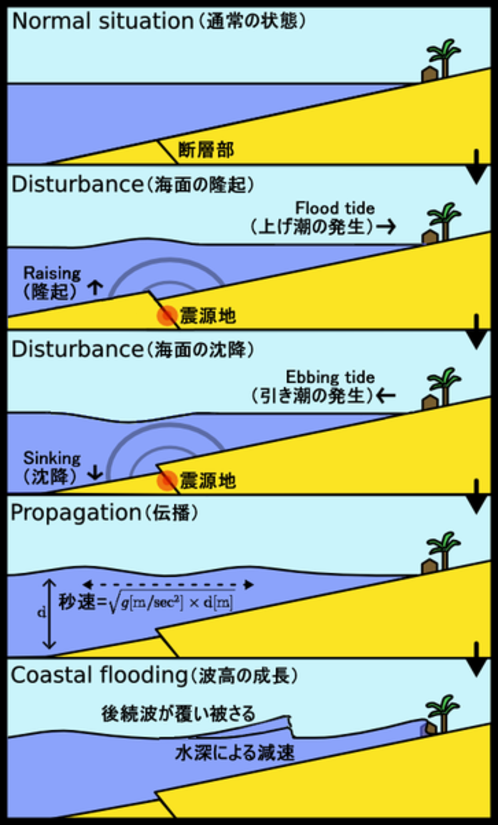
\includegraphics[clip,width=100mm,height=100mm]{eathquack.pdf}
\end{center}
 \caption{津波の発生原理\cite{oka2}}
 \label{fig:eathquack}
\end{figure}

図\ref{fig:eathquack}に地震が起きた際の津波の発生原理を示す.海底で地震が発生すると海底の地盤が動き,海側のプレートと陸側のプレートの隆起と沈降が起こる.プレートの隆起と沈降に合わせて上げ潮や引き潮が発生し,津波につながる.津波は沖から岸に近づくほど波が高くなり,水深が深ければ深いほど速度が早い.

\end{comment}
\newpage


\section{デジタル信号処理}
\subsection{信号処理}
信号処理とは受け取った信号を数理手法で処理する技術や学問のことである.また,アナログ信号処理とデジタル信号処理に分けられ,信号処理を支える基礎的な分野は信号理論とも呼ばれる.

基本的には,信号から信号に変換するものであり,信号とは別の形式の情報を得るものは含まれない.圧縮も含まれないことが多いが,認識や理解,圧縮の前段階としての信号の変換は信号処理と呼ばれることもある.そのため,信号処理はそれらの技術に対して非常に重要であるとともに関連が強い.また,入力と出力が同じ物理量の信号である場合には,フィルタリングとも呼ばれる.

信号処理の主な例としては,音声認識や雑音除去,音声ファイルの圧縮を行う「音響技術」,画像認識やノイズ除去,画像ファイルの圧縮を行う「画像処理」が有名である.

昔までは,高速フーリエ変換,ウェーブレット変換,畳み込み等のアルゴリズムをそれぞれ専用のハードウェアで処理していた.近年ではDSP(Demand-Side Platform)や汎用のハードウェアでソフトウェアで処理したり,FPGA(Field-Plogrammable Gate Array)による再構成可能コンピューティングによって処理する方法が開発されつつある.

\newpage
%
%\subsection{周波数}

\subsection{周波数特性.周波数領域}
周波数とは,1秒あたりに繰り返される波の数で,単位はHzである.主に,音,電気,光,電磁波などに用いられる.
周波数特性とは,周波数と何らかの物理量との関係を表したものである.直流電流ならば単純に比率(ゲイン)だけで伝達特性を定義できる.しかし,実際の被測定物では,周波数によって伝達特性が変化する.さらに交流では比率(ゲイン)だけでなく,入出力間の位相差も問題となる場合が多い.

合成波を時間領域と周波数領域で表したものが図\ref{fig:jikanryouiki},\ref{fig:syuhasuryouiki}になる.
合成波は基本周波数250Hzの$y=1.5\cos2\pi t$,基本周波数50Hzの$y = 4\sin\pi t$,基本周波数150Hzの$y = 3\cos2\pi t$を足し合わせたものになる.
時間領域の図\ref{fig:jikanryouiki}では,X軸を時間,Y軸を振幅で表し,時間とともに変化する波の大きさを表す.一方,周波数領域の図\ref{fig:syuhasuryouiki}では,X軸を周波数,Y軸を波の強さ,または周波数ごとの振幅を表している.


\begin{figure}[htb]
\begin{center}
 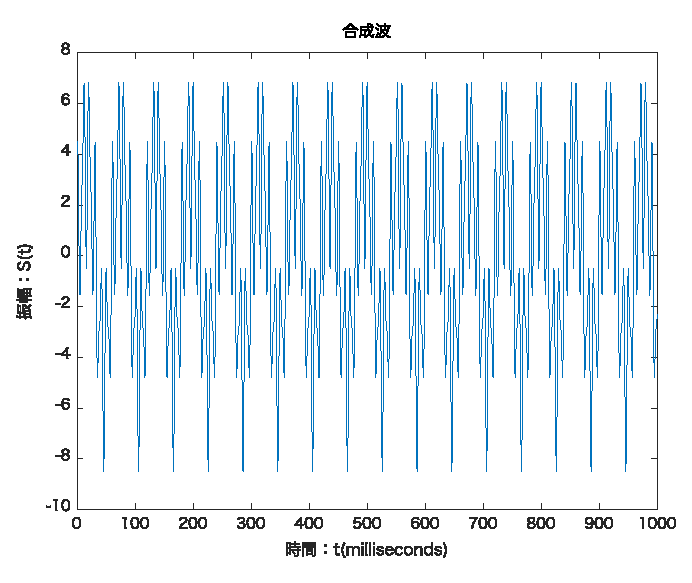
\includegraphics[clip,width=100mm,height=60mm]{sannkakuha.pdf}
\end{center}
 \caption{時間領域における合成波のグラフ}
 \label{fig:jikanryouiki}
\end{figure}
\begin{figure}[htb]
\begin{center}
 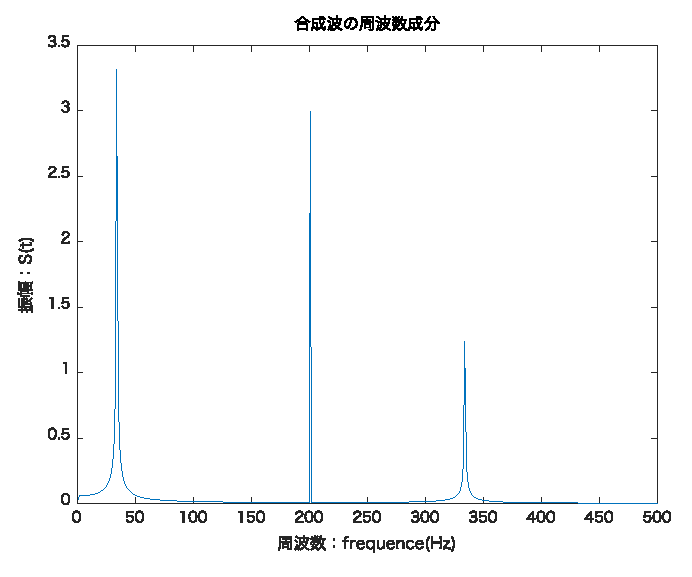
\includegraphics[clip,width=100mm,height=60mm]{sankakuhasyuhasu.pdf}
\end{center}
 \caption{周波数領域における合成波のグラフ}
 \label{fig:syuhasuryouiki}
\end{figure}

信号処理の分野において,時間領域の信号をフーリエ変換したものを周波数特性,または周波数領域と呼ぶ.時間波形から読み取りが困難であっても周波数領域に変換して読み取ることで含まれている波形がわかる.

\subsection{畳み込みと逆畳み込み}
畳み込みとはある関数$g$を平行移動させながら他の関数$f$に重ね足し合わせていく二項演算である.畳み込み積分,合成積,重畳積分,あるいは,コンボリューションとも呼ばれる.画像処理や音響技術においてわざとノイズを付加させるときに使うことが多い.
畳み込みの定義は式(\ref{conv})に示す.

{\Large
\begin{equation}
	\label{conv}
  h(x) =  \int^{\infty}_{-\infty}f(t)g{x-t}dt 
\end{equation}
}
逆畳み込みは,手順としては畳み込みの逆になる.デコンボリューションと呼ばれることもある.画像処理において盲目的なという意味を持つブラインド,逆畳み込みのデコンボリューションをあわせてノイズによって元画像が判別できない状態からノイズ除去をしていく手段としてブラインドデコンボリューションという技術が使われる.近年では,ニューラルネットワークの分野で使われることが多い.
\subsection{ケプストラム法}
ケプストラムとはスペクトルの綴である「spectrum」の最初の4文字を逆にして考案された造語である.ケプストラムとは基本的に周波数特性のIDFTであるため,物理量の次元は時間である.ただし,通常のIDFTと区別するため,ケプストラムの次元は「ケフレンシー(quefrency)」と呼ばれている.これも周波数の綴である「frequency」をもじって考案された造語である\cite{oka4}.

ケプストラム$x_{c}(m)$の定義は$N$は分析窓の長さ,$k$を時間,$m$を周波数で表すと式(\ref{cepst})になる.

{\Large
\begin{dmath}
\label{cepst}
    x_{c}(m) = \frac{1}{N}\sum^{N-1}_{k=0} \log|X(k)|e^{\frac{j2\pi km}{N}} \\
\end{dmath}
}
ただし,範囲$(0\leq m\leq N-1)$になる.

\subsection{パワースペクトルとクロススペクトル}
パワースペクトルとは信号のパワーを一定の周波数帯域に分割し,各帯域ごとのパワーを周波数の関数として表したものをいう.単位は振幅の2乗となる.また,パワースペクトルは波形の周波数成分をエネルギーとして表したものであり,その波形がどれほどのエネルギーを持っているかがわかる\cite{oka6}.

クロススペクトルとは2つの信号のスペクトルのある周波数どうしを掛け合わせたうえで平均化したもので,X軸は周波数,Y軸はパワー($V^2$)で表される.
クロススペクトルがある周波数において大きな値を示していた場合,その周波数において2信号の相関が大きいことがわかる.また,クロススペクトルは伝達関数,相互相関関数,コヒーレンス関数に使われる\cite{oka6}.

\subsection{自己相関と相互相関}
自己相関関数とは,信号がそれ自身を時間シフトした信号とどれだけ良く整合するかを測る尺度であり,時間シフトの大きさの関数として表される.また,信号処理において時間領域信号等の関数または数列を解析されるために用いられる.信号に含まれる繰り返しパターンを探すのに有用である.例えば,ノイズに埋もれた周期的信号の存在を判定したり,信号中の失われた基本周波数を倍音周波数による示唆に基づき同定するために用いられる.

相互相関は2つの信号や配列の類似性を確認するために使われる.関数の配列の結果がすべて1であれば相関があり,すべて0であれば無相関であ理,すべて−1であれば負の相関がある.
2つの信号が、全く同じ場合,自己相関関数と呼び、関数の周期性を調べるのに用いられる. 自己相関関数の値がすべて1のときには、その離散関数の波形の周期性はその関数を表す配列と同じであることがわかる.
\subsection{フーリエ級数展開}
すべての周期信号は基本周波数の正弦波,余弦波,その整数倍の周波数を持つ正弦波,余弦波の重ね合わせとして表現できる.このことから周期信号による音を純音に対して周期信号を重ね合わせとして表現したものを複合音という.
すべての周期信号は式(\ref{furie})のように表すことができる.

{\Large
\begin{equation}
	\label{furie}
  y(t) = a_{0} + \sum^{\infty}_{k=1} (a_{k}\cos k\omega_{0}t +  b_{k}\sin k\omega_{0}t) 
\end{equation}
}

ここで$a_{0}$は直流成分,基本音である角周波数$\omega$の波,$a_{k}$,$b_{k}$は正弦波または余弦波の係数であり,フーリエ係数という.周期信号をこのような正余弦波の成分に展開することをフーリエ級数展開という.
%また,$a_{k}$,$b_{k}$をフーリエ係数という.

\subsection{フーリエ変換}
フーリエ級数展開では,時間的に連続な信号を基本周波数とその倍数の成分の大きさの数字列で表したことになる
しかし,近年ではこのような解析はコンピュータで行うことが主流なので,解析の対象となる信号も連続信号ではなく,時系列と呼ばれる離散的なデータである.また,実際の音の信号を解析する場合は信号の周期を正確に取り出し,解析することは容易ではない.

そこで,実用的な方法として,音の信号を時系列として取り込み,その中から解析したい部分のデータを取り出す.そして,その切り出したデータの長さ分を周期としてみなし,その周期のなす基本周波数とその倍数の成分の係数としてスペクトルを求める.

しかし,このような周期信号は一般的に不連続につながるので,不連続部分が高い周波数の成分として扱われてしまう.そこで窓掛けと呼ばれる処理によって波形の接続部分をなめらかに変形してから解析する.

このように時系列データを周波数のデータ,すなわちスペクトルに変換する方法を離散フーリエ変換(DFT:Discrete Fourier Transform)
という.また,またその逆を離散フーリエ逆変換(IDFT)という.離散フーリエ変換には計算を高速化する手法が開発され,周期とみなすデータ数を2のべき乗に選んだ場合には高速フーリエ変換(FFT:Fast fourier Transform)と呼ばれる方法が使われる\cite{oka3}.

FFTとIFFTを用いることにより時間と周波数の関係を図\ref{fig:fourie}のように示すことができる.
さらに,クロススペクトルの逆フーリエ変換は相互相関関数となる.
%周波数応答関数(伝達関数)の逆フーリエ変換はインパルスレスポンスとなる.
フーリエ変換により数式を変化させることによって,計算しやすい形になることがわかる.

\begin{figure}[h]
\begin{center}
 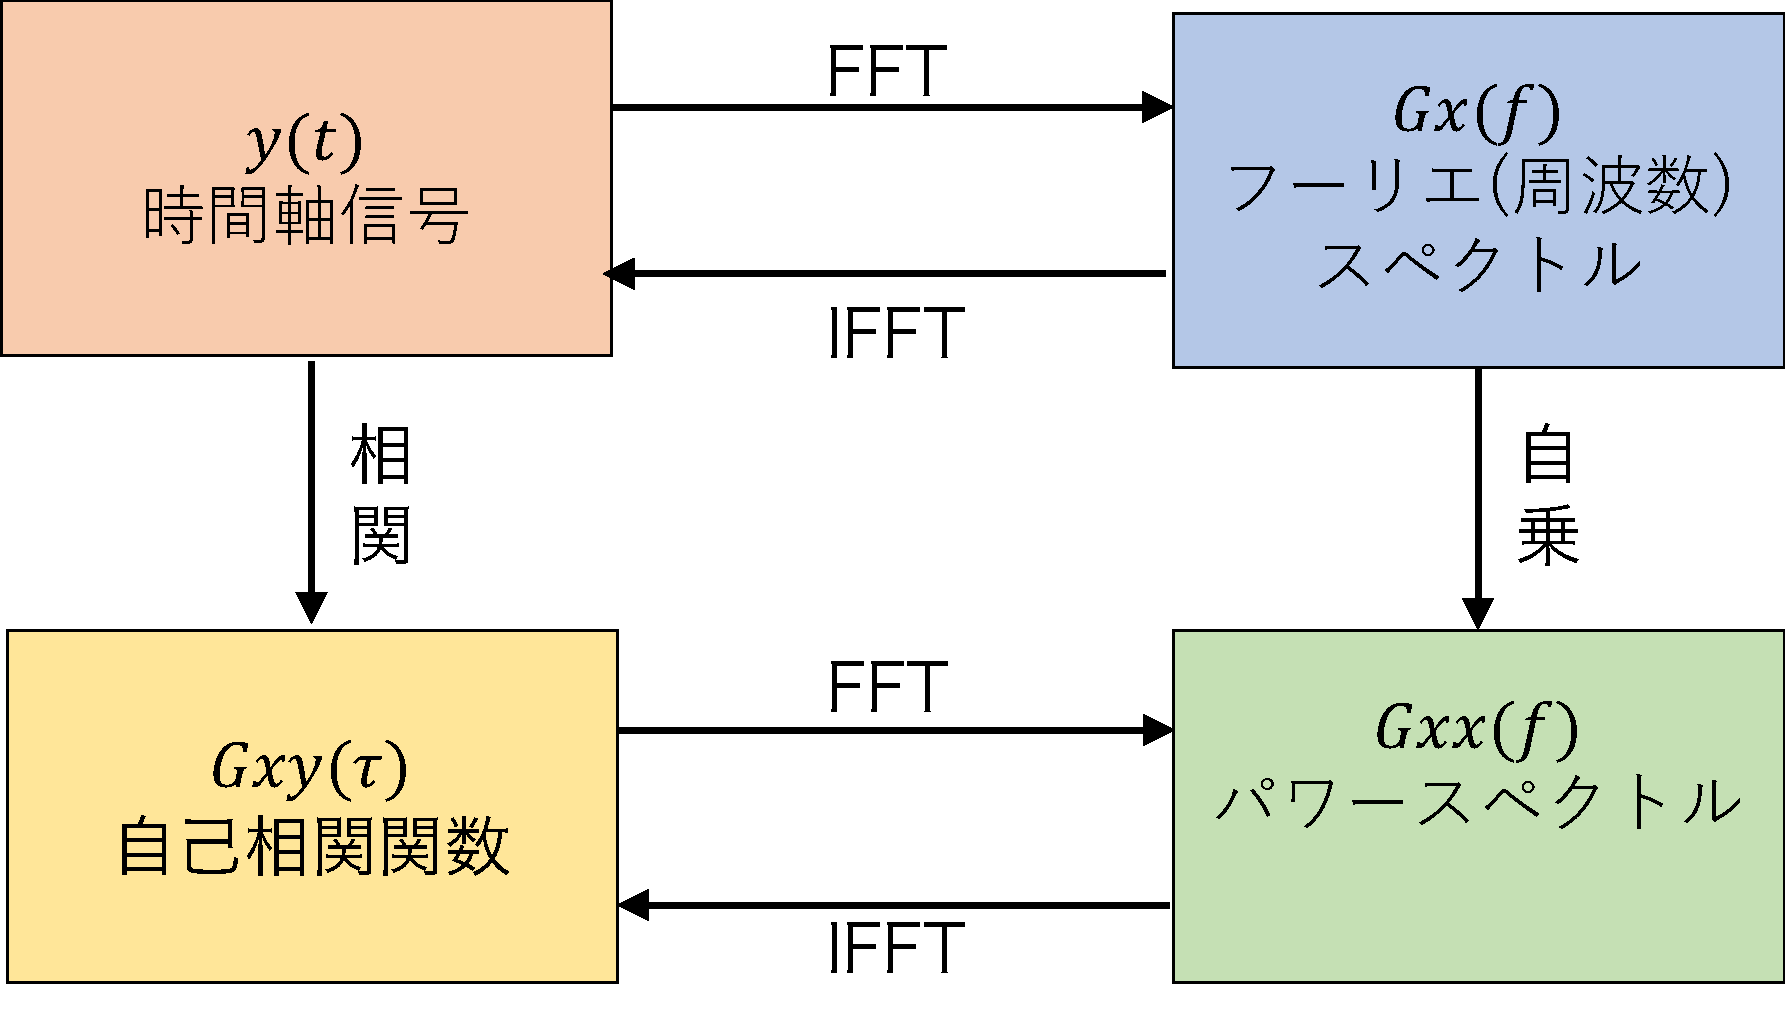
\includegraphics[clip,width=130mm,height=80mm]{fouriesiki.pdf}
\end{center}
 \caption{フーリエ変換が用いられる関係図}
 \label{fig:fourie}
\end{figure}


\newpage

\section{室内音響}
\subsection{残響音・反響}
室内などの閉空間内で発生した音は壁にあたって反射する.反射した音は別の壁による反射を繰り返し,次第に減少していく.このような多重の反射が作り出す現象を残響という.直接音から反射がなくなるまで減衰の包括線は続いていく.
残響により,音声が重複してしまったり,エコーが掛かって聞こえなくなってしまうことがある.
その様子を波形にしたものを図\ref{fig:hakei}に示す.
上の波形が残響がないもの下の波形が残響があるものになる.音声を聞くと,こもったような音になってしまい音節と音節が重なる瞬間が出てきてしまうため聞き取りづらいのがわかる.
% 図5.1-1
\begin{figure}[h]
\begin{center}
 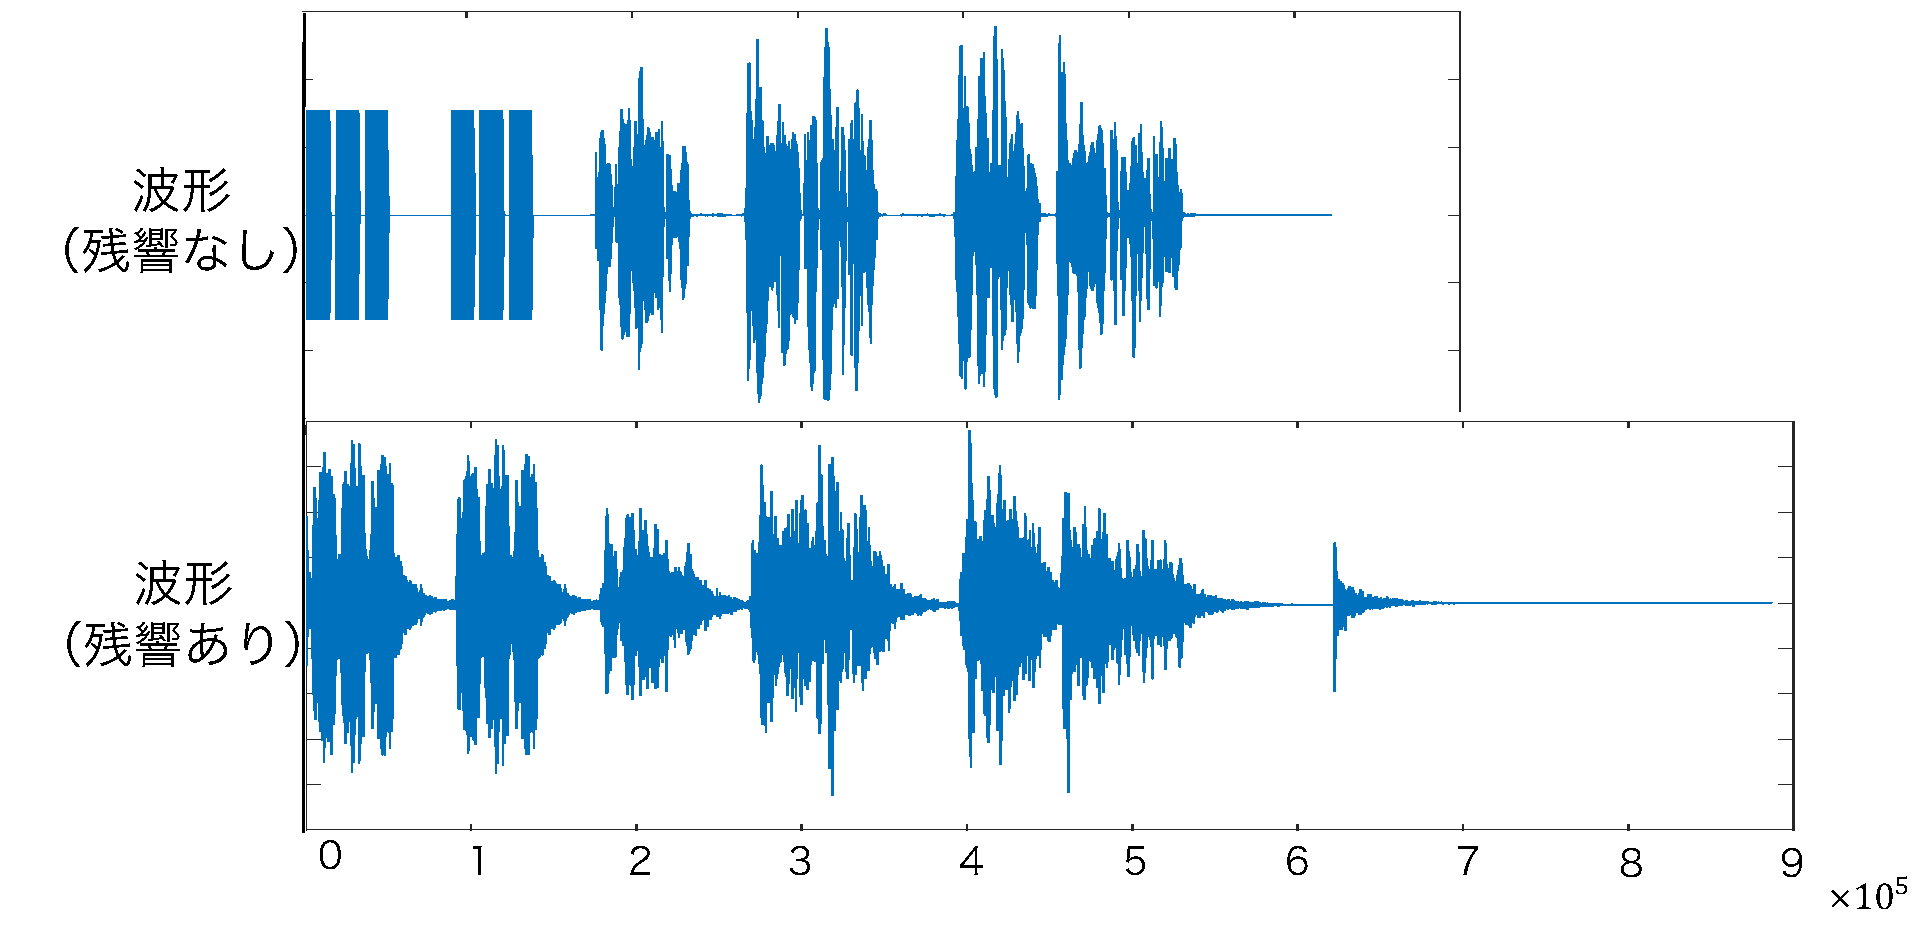
\includegraphics[clip,width=130mm,height=80mm]{hakeikekka.pdf}
\end{center}
 \caption{残響影響波形例}
 \label{fig:hakei}
\end{figure}

\newpage

\subsection{インパルス応答}
音源から単一の衝撃音を発したときの受音点での音の観測結果の例を図\ref{fig:impulse},波形の例を図\ref{fig:impulse1}に示す.直接音(インパルス)に対し,初期反射,高次反射と続いていくのが図\ref{fig:impulse}から読み取れる.反射音は反射を繰り返すたびに音の大きさが小さくなっていくのが分かる.それぞれの反射の音の大きさの最大を結んだ線を減衰の包括線という.直接音,反射音すべてを含む空間情報をインパルス応答と呼ぶ\cite{oka3}.

% 図5.2-1
\begin{figure}[h]
\begin{center}
 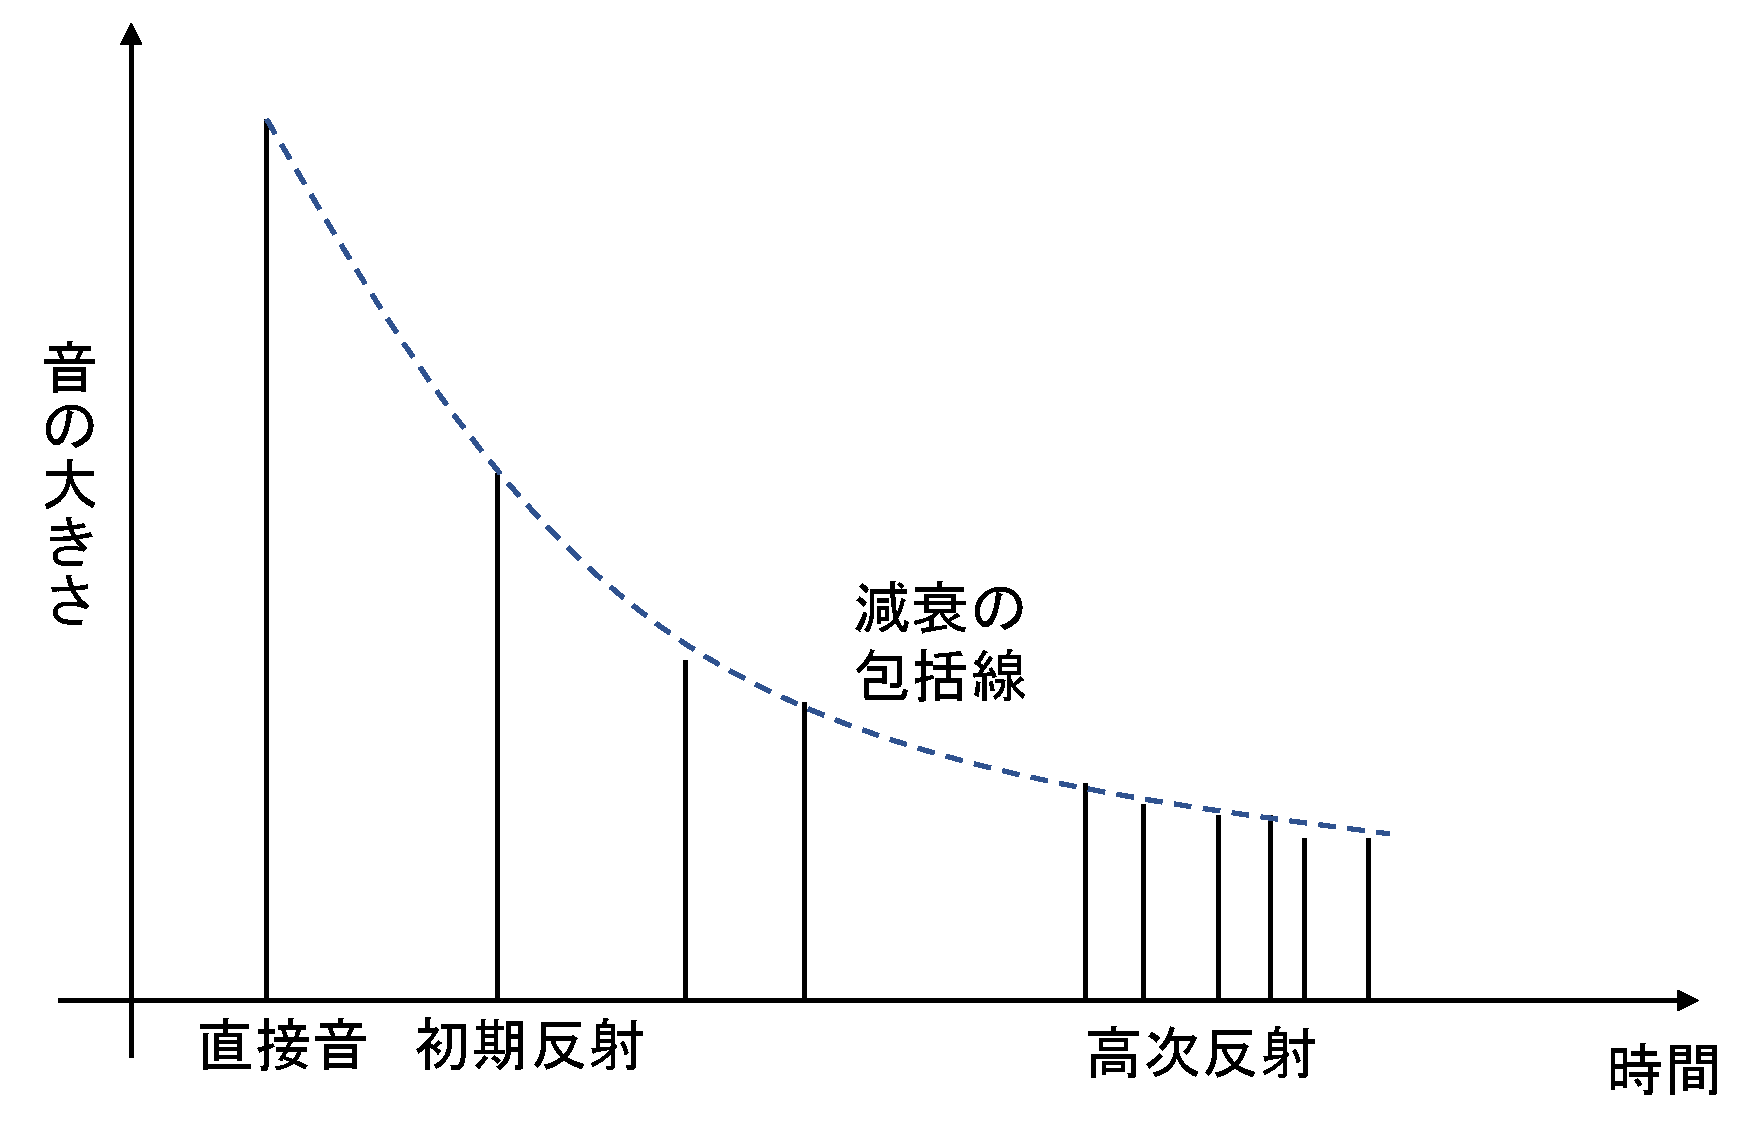
\includegraphics[clip,width=140mm,height=80mm]{ImpulseResponse.pdf}
\end{center}
 \caption{インパルス応答の例\cite{oka3}}
 \label{fig:impulse}
\end{figure}

\begin{figure}[h]
\begin{center}
 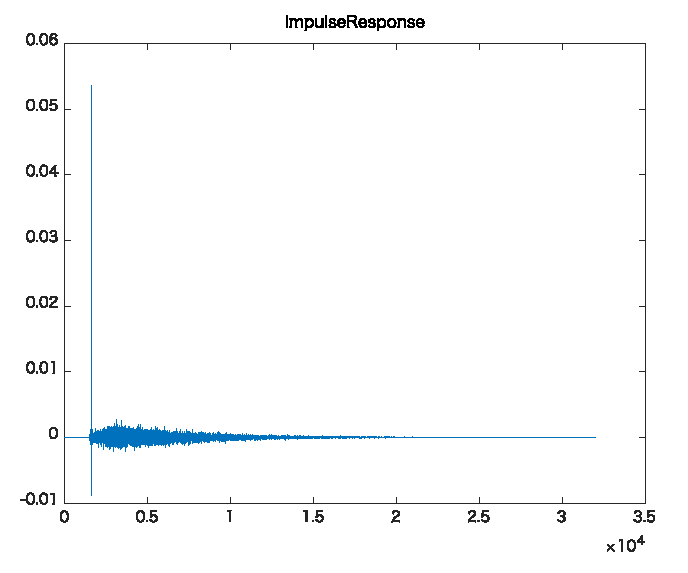
\includegraphics[clip,width=85mm,height=60mm]{imprps.pdf}
\end{center}
 \caption{インパルス応答の波形例}
 \label{fig:impulse1}
\end{figure}
\newpage
\subsection{ランダム信号を用いたインパルス信号測定法}
信号の継続時間はインパルス信号に比べて桁違いに長いので,S/Nの良い,つまり精度の良い測定が期待できるはずである.
図(\ref{fig:impsystem})のように,システムへの入力信号を$x(t)$,出力信号を$y(t)$と表したとき,両者は畳み込み記号*を用いて以下の関係で結び付けられるとする.
{\Large
\begin{equation}
\label{impulse}
  y(t) = h(t)*x(t)=\int^{\infty}_{-\infty} h(t)(t - \tau){d\tau}
\end{equation}
}
システムのインパルス応答$h(t)$を求めるために直接相関法,クロススペクトル推定法がある.

\begin{figure}[h]
\begin{center}
 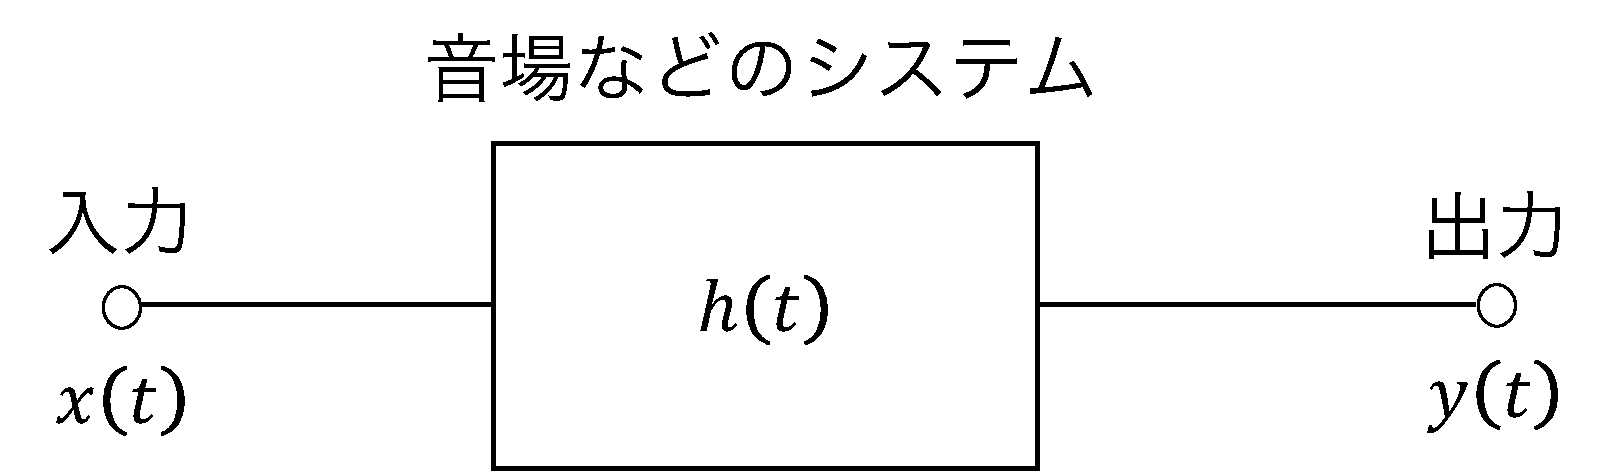
\includegraphics[clip,width=70mm,height=30mm]{impsystem.pdf}
\end{center}
 \caption{入力$x(t)$,システム$h(t)$,および出力$y(t)$の関係}
 \label{fig:impsystem}
\end{figure}

\newpage

\subsubsection{直接相関法}
\label{sec:直接相関法}
入力信号$x(t)$の自己相関関数$R_x(\tau)$および出力信号$y(t)$との相互相関関数$R_{xy}(\tau)$は期待値$E[]$を用いて式(\ref{jikosoukan}),(\ref{sougosoukan})のように表される.

{\Large
\begin{equation}
\label{jikosoukan}
  R_x(\tau) =E[x(t)x(t+\tau)]=\lim_{T \to \infty}\frac{1}{T} \int^{T}_{0}x(t)x(t+\tau){dt}
\end{equation}
}

{\Large
\begin{equation}
\label{sougosoukan}
   R_{xy}(\tau) =E[x(t)y(t+\tau)]=\lim_{T \to \infty}\frac{1}{T} \int^{T}_{0}x(t)y(t+\tau){dt}
\end{equation}
}
ただし,$E[x(t)x(t+\tau)]$は$x(t)x(t+\tau)$の期待値(時間平均)を求めるという意味である.ここで$R_{xy}$を式(\ref{henkei})のように変形する.

{\Large
\begin{dmath}
\label{henkei}
   R_{xy}(\tau) = E[x(t)\int^{\infty}_{-\infty}h(\tau_1)x(t+\tau-\tau_1){d\tau_1}] \nonumber \\ \\
   =\int^{\infty}_{-\infty}h(\tau_1)E[x(t)x(t+\tau-\tau_1)dt]{d\tau_1} \nonumber \\ \\ 
   =\int^{\infty}_{-\infty}h(\tau_1)R_x(\tau-\tau_1){d\tau_1} \nonumber \\ \\
   =h(\tau)*R_x(\tau)
\end{dmath}
}

つまり,入力信号$x(t)$と出力信号$y(t)$の相互相関関数$R_{xy}(\tau)$は,入力信号の自己相関関数$R_x(\tau)$とシステムのインパルス応答$h(\tau)$の畳み込みで表される.

ここで,入力信号として自己相関関数がデルタ関数であるような信号を用いれば,自己相関関数を求めることでそのまま,システムのインパルス応答が求められることになる.つまり,$R_x(\tau)=\delta(\tau)$である関数を用いれば良い.この目的のために,ホワイトノイズなどを用いることができる.この方法による測定で,外部からの無相関のノイズが混入した場合のことを考察する.ノイズ込みの出力波形をノイズを$n(t)$とし,$y'=y(t)+n(t)$とすると,

{\Large
\begin{dmath}
\label{henkei2}
   R_{xy'}(\tau) =E[x(t)y'(t+\tau)]=E[x(t)y{(y(t+\tau)+n(t+\tau)}] \\
   =E[x(t)y(t+\tau)]+E[x(t)n(t+\tau)]
\end{dmath}
}

となり,一般的に右辺第2項に含まれるノイズは無相関であるため,無相関の期待値は0になる.そのため,右辺第2項は0と考えられるために,

{\Large
\begin{equation}
\label{ketsuron}
   R_{xy'}(\tau) =E[x(t)y(t+\tau)]=R_{xy'}(\tau)
\end{equation}
}

となり,原理的にこの方法はノイズの影響を受けないことがわかる.

\subsubsection{クロススペクトル推定法}
\label{sec:クロススペクトル推定法}
自己相関関数,相互相関数をフーリエ変換することで,それぞれのパワースペクトル密度関数$S_x(f)$,クロススペクトル密度$S_{xy}(f)$が得られる.これを式で書くと,式(\ref{powerspec}),(\ref{crossspec})のようになる.

{\Large
\begin{equation}
\label{powerspec}
  S_x(f) = \int^{\infty}_{-\infty} R_x(\tau)e^{-j\omega \tau}{d\tau}
\end{equation}
}

{\Large
\begin{equation}
\label{crossspec}
  S_{xy}(f) = \int^{\infty}_{-\infty} R_{xy}(\tau)e^{-j\omega \tau}{d\tau}
\end{equation}
}

更に時間領域の畳み込みの関係が周波数領域では積となる合成積則より,\ref{sec:直接相関法}の式(\ref{henkei})以下の流れと等しくなる.

{\Large
\begin{equation}
\label{crossspec1}
  S_{xy}(f) = H(f)\cdot S_x(f)
\end{equation}
}

ここに$H(f)$はインパルス応答の周波数領域表現である.

したがって,

{\Large
\begin{equation}
\label{crossspec2}
  H(f) = \frac {S_{xy}(f)}{S_x(f)}
\end{equation}
}
を求め,これを逆フーリエ変換することでインパルス応答が求められることになる.ここで,パワースペクトル密度と信号のフーリエ変換の関係により複素共役である$X^{*}$を用いて,
{\Large
\begin{equation}
\label{crossspec3}
  S_{x}(f) = E[X^{*}(f)X(f)]
\end{equation}
}

{\Large
\begin{equation}
\label{crossspec4}
  S_{xy}(f) = E[X^{*}(f)Y(f)]
\end{equation}
}
\subsection{伝達関数}
伝達関数とはシステムへの入力を出力に変換する関数のことをいう.伝達関数は,すべての初期値を0としたときの,制御系の出力と入力のラプラス変換(またはZ変換)の比で表される.すなわち,連続システムのとき,出力信号$y(t)$のラプラス変換を$Y(s)$,入力信号$x(t)$のラプラス変換を$X(s)$とすれば,伝達関数$G(s)$は
{\Large
\begin{equation}
	\label{noref}
  G(s) =  \frac{Y(s)}{X(s)} = \frac{{\int^{\infty}_0}y(t)e^{-st}{dt}}{{\int^{\infty}_0}x(t)e^{-st}{dt}}
\end{equation}
}


と表される.
離散システムに対して,伝達関数はZ変換によって,
{\Large
\begin{equation}
	\label{noref}
  H(z) =   \frac{Y(z)}{X(z)} = \frac{{\sum^{\infty}_{n = -\infty}}y(n)Z^{-n}}{{\sum^{\infty}_{n = -\infty}}x(n)Z^{-n}}
\end{equation}
}


と表される.$z$は一般の複素数であり,$z=e^{\sigma +j\omega T} =re^{j\omega T}$,$r=e^{\sigma}$のように表せる.

この伝達関数法では,時間領域の関数を,ラプラス変換(またはZ変換)によって複素平面に写像を取り,さらに周波数領域に変換することにより,系の特性や安定性を解析するのに用いる.ただし,対象となる系が1入力1出力(線形関数)に限られているため,複雑な系(多入力多出力,非線形)の解析には状態空間法を用いる.

インパルス応答をフーリエ変換したものを伝達関数という.


\newpage

\subsection{ノイズ}
ノイズとは,処理対象となる情報以外の不要な情報のことである.歴史的理由から雑音に代表されるため,しばしば工学分野の文章では音以外に関しても「雑音」と訳したり表現したりして,音以外の信号等におけるノイズの意味で扱っていることがある.マイク録音を行ったときに不用意な音まで録音されてしまうことがある.それらの不要な成分を総称してノイズと呼ぶ.ノイズは正確な音声信号処理を阻害する要因となるため除去するのが望ましいが,非常に不規則な値を取るため手がかりなしで適切に除去することは困難である.

不規則なノイズに対して,統計的な性質を知ることが重要であり,ホワイトノイズはすべての周波数で同じ強度となるため,四角のような形をしていることが多い.ノイズの音としては「シャー」という音となる.また,代表的なモデルとして頻繁に使用される.
ホワイトノイズ例を図\ref{fig:whitenoize}に示す.

% 図5.4-1
\begin{figure}[h]
\begin{center}
 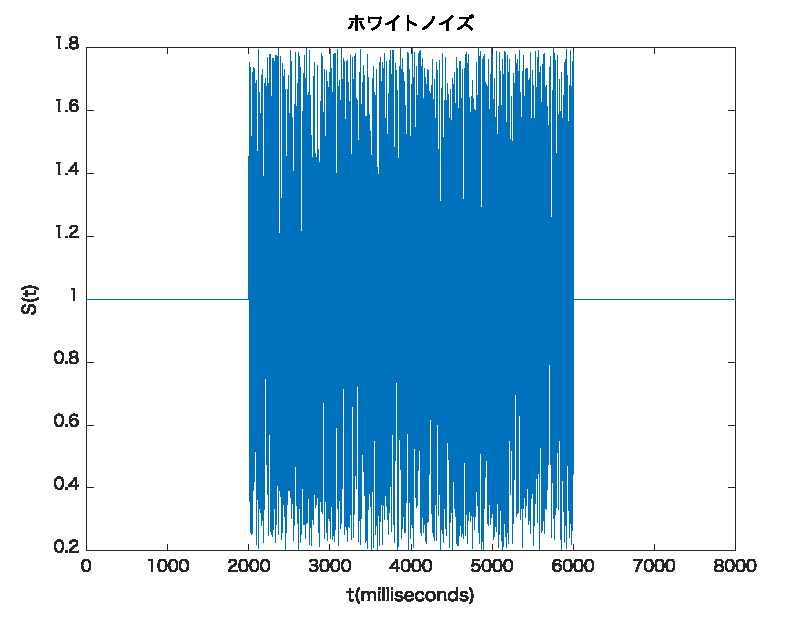
\includegraphics[clip,width=85mm,height=65mm]{whitenoize.pdf}
\end{center}
 \caption{ホワイトノイズ}
 \label{fig:whitenoize}
\end{figure}


\subsection{残響推定方法}
残響推定方法には2種類あり,ノイズ断続法とインパルス応答積分法の2つになる.
\begin{description}
   \item[1.ノイズ断続法]\mbox{}\\
            この手法は,スピーカから試験音を放射し,試験音が部屋に充満したら,音を停止した後の音圧レベルを記録して残響時間を読み取る方法である.
   \item[2.インパルス応答積分法]\mbox{}\\
	    この手法は,測定した音源点と受音点間のインパルス応答から求めた残響減衰曲線の傾きで残響時間を推定する方法である.
\end{description}
\begin{comment}

\subsubsection{ノイズ断続法}
この手法は,スピーカから試験音を放射し,試験音が部屋に充満したら,音を停止した後の音圧レベルを記録して残響時間を読み取る方法である.
\subsubsection{インパルス応答積分法}
この手法は,測定した音源点と受音点間のインパルス応答から求めた残響減衰曲線の傾きで残響時間を推定する方法である.
\end{comment}

\newpage

\section{残響除去の提案}
\begin{comment}
\subsection{パワースペクトルとクロススペクトル}
パワースペクトルとは信号のパワーを一定の周波数帯域に分割し,各帯域ごとのパワーを周波数の関数として表したものをいう.単位は振幅の2乗となる.また,パワースペクトルは波形の周波数成分をエネルギーとして表したものであり,その波形がどれほどのエネルギーを持っているかがわかる\cite{oka6}.

クロススペクトルとは2つの信号のスペクトルのある周波数どうしを掛け合わせたうえで平均化したもので,X軸は周波数,Y軸はパワー($V^2$)で表される.
クロススペクトルがある周波数において大きな値を示していた場合,その周波数において2信号の相関が大きいことがわかる.また,クロススペクトルは伝達関数,相互相関関数,コヒーレンス関数に使われる\cite{oka6}.

\end{comment}

\begin{comment}

\subsection{畳み込みと逆畳み込み}
畳み込みとはある関数$g$を平行移動させながら他の関数$f$に重ね足し合わせていく二項演算である.畳み込み積分,合成積,重畳積分,あるいは,コンボリューションとも呼ばれる.画像処理や音響技術においてわざとノイズを付加させるときに使うことが多い.
畳み込みの定義は式(\ref{conv})に示す.

{\Large
\begin{equation}
	\label{conv}
  h(x) =  \int^{\infty}_{-\infty}f(t)g{x-t}dt 
\end{equation}
}
逆畳み込みは,手順としては畳み込みの逆になる.デコンボリューションと呼ばれることもある.画像処理において盲目的なという意味を持つブラインド,逆畳み込みのデコンボリューションをあわせてノイズによって元画像が判別できない状態からノイズ除去をしていく手段としてブラインドデコンボリューションという技術が使われる.近年では,ニューラルネットワークの分野で使われることが多い.
\subsection{ケプストラム法}
ケプストラムとはスペクトルの綴である「spectrum」の最初の4文字を逆にして考案された造語である.ケプストラムとは基本的に周波数特性のIDFTであるため,物理量の次元は時間である.ただし,通常のIDFTと区別するため,ケプストラムの次元は「ケフレンシー(quefrency)」と呼ばれている.これも周波数の綴である「frequency」をもじって考案された造語である\cite{oka4}.

ケプストラム$x_{c}(m)$の定義は$N$は分析窓の長さ,$k$を時間,$m$を周波数で表すと式(\ref{cepst})になる.

{\Large
\begin{dmath}
\label{cepst}
    x_{c}(m) = \frac{1}{N}\sum^{N-1}_{k=0} \log|X(k)|e^{\frac{j2\pi km}{N}} \\
\end{dmath}
}
ただし,範囲$(0\leq m\leq N-1)$になる.
\end{comment}
\begin{comment}

\subsection{ランダム信号を用いたインパルス信号測定法}
信号の継続時間はインパルス信号に比べて桁違いに長いので,S/Nの良い,つまり精度の良い測定が期待できるはずである.
図(\ref{fig:impsystem})のように,システムへの入力信号を$x(t)$,出力信号を$y(t)$と表したとき,両者は畳み込み記号*を用いて以下の関係で結び付けられるとする.
{\Large
\begin{equation}
\label{impulse}
  y(t) = h(t)*x(t)=\int^{\infty}_{-\infty} h(t)(t - \tau){d\tau}
\end{equation}
}
システムのインパルス応答$h(t)$を求めるために直接相関法,クロススペクトル推定法がある.

\begin{figure}[h]
\begin{center}
 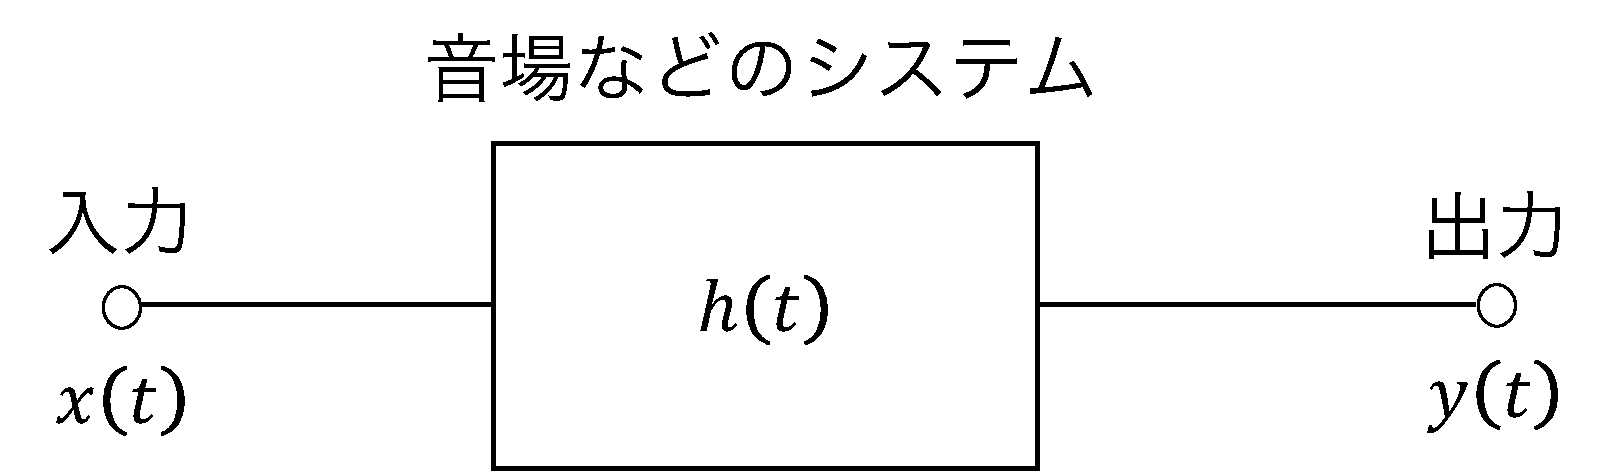
\includegraphics[clip,width=70mm,height=30mm]{impsystem.pdf}
\end{center}
 \caption{入力$x(t)$,システム$h(t)$,および出力$y(t)$の関係}
 \label{fig:impsystem}
\end{figure}

\newpage

\subsubsection{直接相関法}
\label{sec:直接相関法}
入力信号$x(t)$の自己相関関数$R_x(\tau)$および出力信号$y(t)$との相互相関関数$R_{xy}(\tau)$は期待値$E[]$を用いて式(\ref{jikosoukan}),(\ref{sougosoukan})のように表される.

{\Large
\begin{equation}
\label{jikosoukan}
  R_x(\tau) =E[x(t)x(t+\tau)]=\lim_{T \to \infty}\frac{1}{T} \int^{T}_{0}x(t)x(t+\tau){dt}
\end{equation}
}

{\Large
\begin{equation}
\label{sougosoukan}
   R_{xy}(\tau) =E[x(t)y(t+\tau)]=\lim_{T \to \infty}\frac{1}{T} \int^{T}_{0}x(t)y(t+\tau){dt}
\end{equation}
}
ただし,$E[x(t)x(t+\tau)]$は$x(t)x(t+\tau)$の期待値(時間平均)を求めるという意味である.ここで$R_{xy}$を式(\ref{henkei})のように変形する.

{\Large
\begin{dmath}
\label{henkei}
   R_{xy}(\tau) = E[x(t)\int^{\infty}_{-\infty}h(\tau_1)x(t+\tau-\tau_1){d\tau_1}] \nonumber \\ \\
   =\int^{\infty}_{-\infty}h(\tau_1)E[x(t)x(t+\tau-\tau_1)dt]{d\tau_1} \nonumber \\ \\ 
   =\int^{\infty}_{-\infty}h(\tau_1)R_x(\tau-\tau_1){d\tau_1} \nonumber \\ \\
   =h(\tau)*R_x(\tau)
\end{dmath}
}

つまり,入力信号$x(t)$と出力信号$y(t)$の相互相関関数$R_{xy}(\tau)$は,入力信号の自己相関関数$R_x(\tau)$とシステムのインパルス応答$h(\tau)$の畳み込みで表される.

ここで,入力信号として自己相関関数がデルタ関数であるような信号を用いれば,自己相関関数を求めることでそのまま,システムのインパルス応答が求められることになる.つまり,$R_x(\tau)=\delta(\tau)$である関数を用いれば良い.この目的のために,ホワイトノイズなどを用いることができる.この方法による測定で,外部からの無相関のノイズが混入した場合のことを考察する.ノイズ込みの出力波形をノイズを$n(t)$とし,$y'=y(t)+n(t)$とすると,

{\Large
\begin{dmath}
\label{henkei2}
   R_{xy'}(\tau) =E[x(t)y'(t+\tau)]=E[x(t)y{(y(t+\tau)+n(t+\tau)}] \\
   =E[x(t)y(t+\tau)]+E[x(t)n(t+\tau)]
\end{dmath}
}

となり,一般的に右辺第2項に含まれるノイズは無相関であるため,無相関の期待値は0になる.そのため,右辺第2項は0と考えられるために,

{\Large
\begin{equation}
\label{ketsuron}
   R_{xy'}(\tau) =E[x(t)y(t+\tau)]=R_{xy'}(\tau)
\end{equation}
}

となり,原理的にこの方法はノイズの影響を受けないことがわかる.

\subsubsection{クロススペクトル推定法}
\label{sec:クロススペクトル推定法}
自己相関関数,相互相関数をフーリエ変換することで,それぞれのパワースペクトル密度関数$S_x(f)$,クロススペクトル密度$S_{xy}(f)$が得られる.これを式で書くと,式(\ref{powerspec}),(\ref{crossspec})のようになる.

{\Large
\begin{equation}
\label{powerspec}
  S_x(f) = \int^{\infty}_{-\infty} R_x(\tau)e^{-j\omega \tau}{d\tau}
\end{equation}
}

{\Large
\begin{equation}
\label{crossspec}
  S_{xy}(f) = \int^{\infty}_{-\infty} R_{xy}(\tau)e^{-j\omega \tau}{d\tau}
\end{equation}
}

更に時間領域の畳み込みの関係が周波数領域では積となる合成積則より,\ref{sec:直接相関法}の式(\ref{henkei})以下の流れと等しくなる.

{\Large
\begin{equation}
\label{crossspec1}
  S_{xy}(f) = H(f)\cdot S_x(f)
\end{equation}
}

ここに$H(f)$はインパルス応答の周波数領域表現である.

したがって,

{\Large
\begin{equation}
\label{crossspec2}
  H(f) = \frac {S_{xy}(f)}{S_x(f)}
\end{equation}
}
を求め,これを逆フーリエ変換することでインパルス応答が求められることになる.ここで,パワースペクトル密度と信号のフーリエ変換の関係により複素共役である$X^{*}$を用いて,
{\Large
\begin{equation}
\label{crossspec3}
  S_{x}(f) = E[X^{*}(f)X(f)]
\end{equation}
}

{\Large
\begin{equation}
\label{crossspec4}
  S_{xy}(f) = E[X^{*}(f)Y(f)]
\end{equation}
}

となることになる.つまり,観測した信号$x(t)$,$y(t)$か,実際にはその離散時間表現$x(n)$,$y(n)$のフーリエ変換を求めて,上記の演算を行うことでインパルス応答の推定が行えることになる.フーリエ変換を用いることができる,ということは演算時間短縮に関する大きなメリットにもなる.

\end{comment}

\subsection{先行研究と提案手法}
\subsubsection{先行研究による手法}
非常放送には反射音が建物などにより付加してしまい内容を聞き取りづらいといったことが問題点として挙げられている.その反射音を除去するために佐藤はクロススペクトル法を用いて残響の除去に取り組んだ.

手法の構想図を図\ref{fig:手法構想図}に示す
手法としては元波形の前におらかじめ信号音を付加させておき,それをもとに残響度合いを推定するため,インパルス応答を求める.反射音の付加された音声をインパルス応答で割ることで残響が除去できる.残響を除去した音声をユーザの使用するモバイルデバイスによりリアルタイムにクリアな音声を聞き取る手法である.
\begin{figure}[h]
\begin{center}
 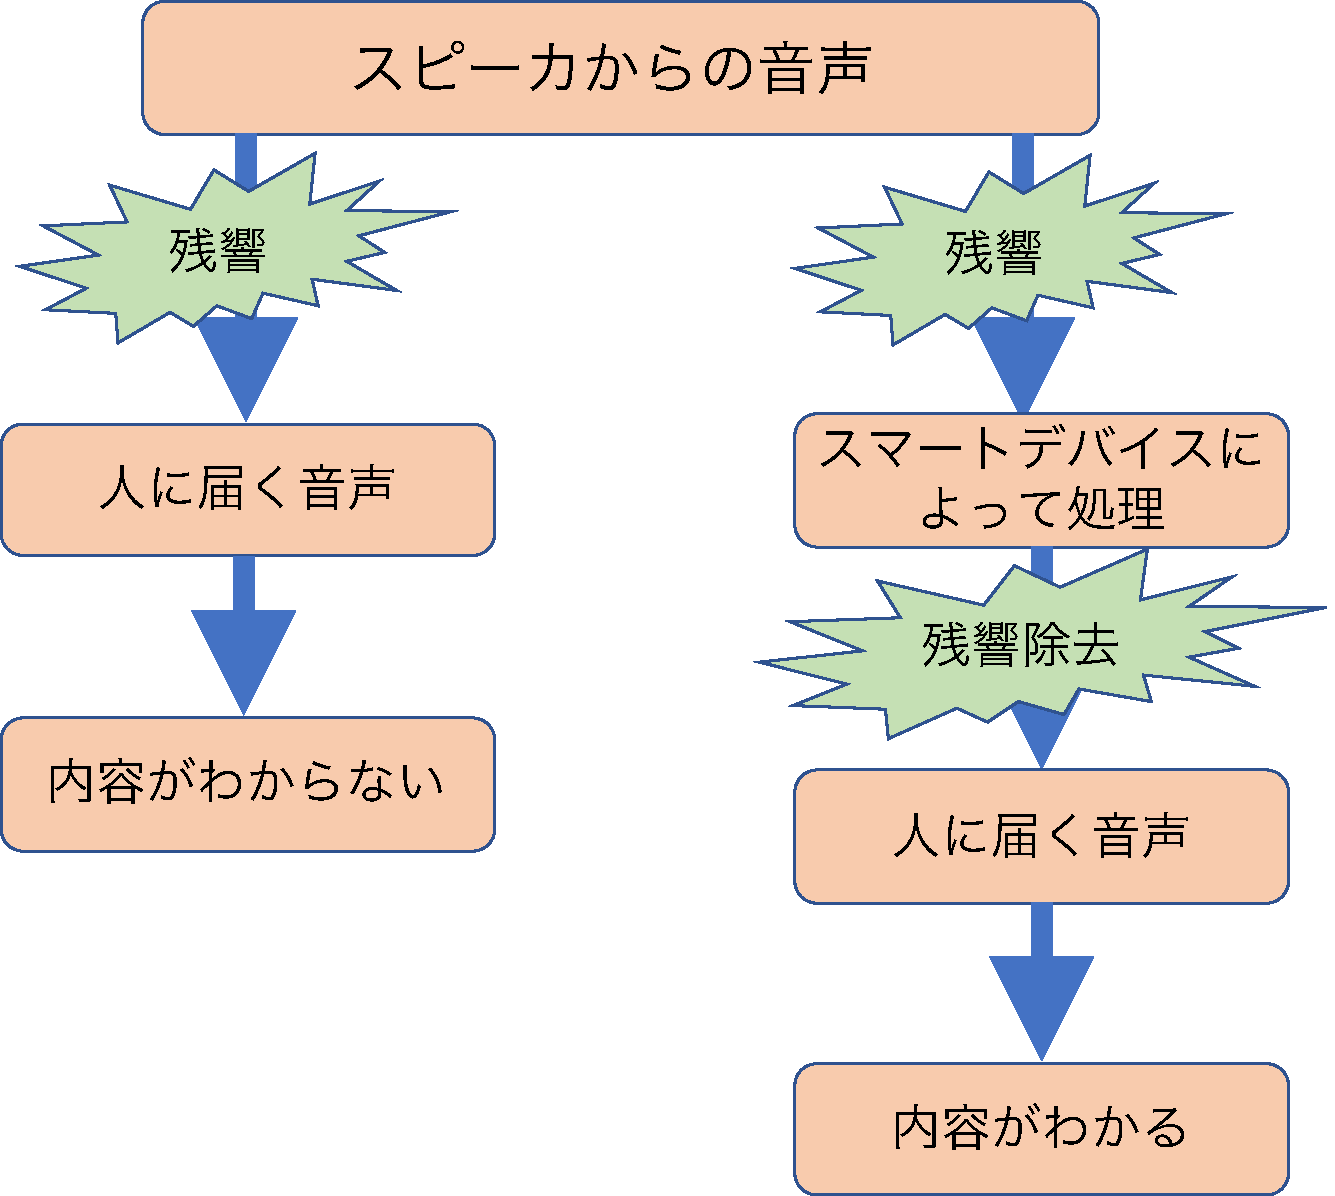
\includegraphics[clip,width=100mm,height=100mm]{risouzu.pdf}
\end{center}
 \caption{先行研究手法構想図}
 \label{fig:手法構想図}
\end{figure}

\begin{comment}
\newpage
先頭に付加させた信号音を図\ref{fig:信号音}に示す.「ピーピーピー」という音が2回繰り返される3秒程度の信号音になる.緊急地震速報に付加しているものを参考に作成した.
\begin{figure}[h]
\begin{center}
 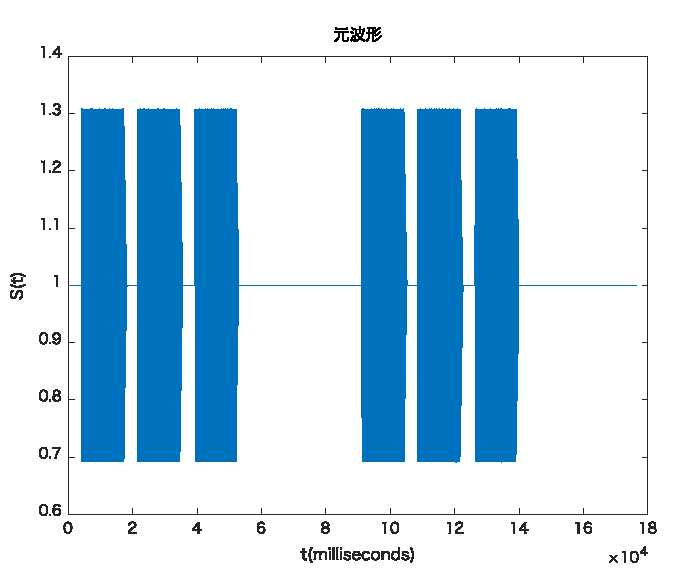
\includegraphics[clip,width=130mm,height=80mm]{sinngouon.pdf}
\end{center}
 \caption{信号音}
 \label{fig:信号音}
\end{figure}

\end{comment}

\newpage
\subsubsection{先行研究の計算内容}
計算内容としては元波形を$S(t)$,反射音の含まれた音声を$R(t)$とすると,
はじめに両波形をフーリエ変換することにより周波数成分$S(f)$$R(f)$を求める.

{\Large
\begin{equation}
\label{先行研究最初}
  S(f) = \int^{\infty}_{-\infty}S(t)e^{(-j2\pi f)}dt \\
\end{equation}
}

{\Large
\begin{equation}
  R(f) = \int^{\infty}_{-\infty}R(t)e^{(-j2\pi f)}dt \\
\end{equation}
}
元波形の周波数成分を二乗することでパワースペクトル$P(f)$を求めることができる.

{\Large
\begin{equation}
	\label{power}
  P(f) = (S(f))^2
\end{equation}
}

元波形の周波数成分と反射音の含んだ波形の周波数成分の積によりクロススペクトル$C(f)$を求めることができる.
{\Large
\begin{equation}
	\label{cross}
  C(f) = S(f)・R(f)
\end{equation}
}

クロススペクトルをパワースペクトルで除算することにより伝達関数$H(f)$を求めることができる.

{\Large
\begin{equation}
	\label{transfer}
  H(f) = \frac{C(f)}{P(f)}
\end{equation}
\normalsize}

伝達関数を逆フーリエ変換することによりインパルス応答$IR(t)$を求めることができる.

{\Large
\begin{equation}
	\label{IR}
  IR(t) =  \int^{\infty}_{-\infty}H(f)e^{(j2\pi f)}dt 
\end{equation}
}

求めたインパルス応答を用いて,反射音の付加している音声の周波数成分をインパルス応答で除算することにより反射音の除去された音声の周波数成分$N(f)$を求めることができる.

{\Large
\begin{equation}
	\label{norefcomp}
  N(f) = \frac{R(f)}{IR(t)}
\end{equation}
}

またそれを逆フーリエ変換することにより反射音の除去された音声$N(t)$を取り出すことができる.

{\Large
\begin{equation}
	\label{noref}
  N(t) =  \int^{\infty}_{-\infty}N(f)e^{(j2\pi f)}dt 
\end{equation}
}

式(\ref{先行研究最初})\textasciitilde(\ref{noref})より元信号$S(t)$と提案手法によって求めた$N(t)$が同等である.

{\Large
\begin{equation}
  N(t)\simeq S(t)
\end{equation}
}



\subsubsection{先行研究が動作しなかった考察}
式\ref{norefcomp}において残響を含む波形の周波数成分$R(f)$とインパルス応答$IR(t)$の計算が時間領域と周波数領域の計算になるため,領域が一致していない.
また,先行研究の計算内容をもとに実音声を用いて除去を試みた.結果,波形が全く違うものになってしまい,音声を聞いても「プツッ」という音声が流れるのみになってしまった.


\newpage
\subsection{提案手法}
本研究では,先行研究と同じように予め波形の先頭に信号音を付加させておく.その信号音をもとに残響を除去する.残響を除去した音声をユーザの使用するモバイルデバイスによりリアルタイムにクリアな音声を聞き取る手法である.残響を除去する手法は反射音が直接音に畳み込まれているものとして,反射音を付加した音声を元信号で逆畳み込みをすることで反射音を求められると考えた.また,反射音が付加されている音声から反射音を除去するために信号同士の計算が簡単になるケプストラム法を用いて反射音の除去された信号の抽出が可能である.

先頭に付加させた信号音を図\ref{fig:信号音}に示す.「ピーピーピー」という音が2回繰り返される3秒程度の信号音になる.緊急地震速報に付加しているものを参考に作成した.
\begin{figure}[h]
\begin{center}
 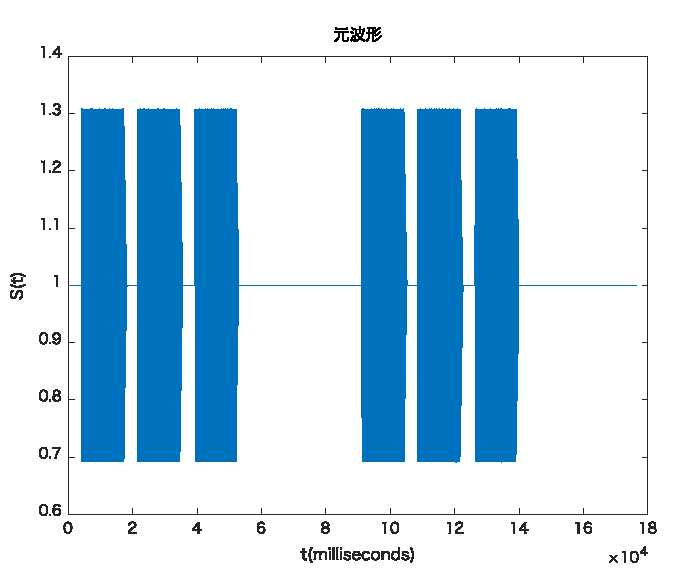
\includegraphics[clip,width=100mm,height=70mm]{sinngouon.pdf}
\end{center}
 \caption{信号音}
 \label{fig:信号音}
\end{figure}

\newpage

逆畳み込みによって求められた反射音D$(t)$,反射音が含まれた音声R$(t)$,放送内容の音声S$(t)$
とすると図\ref{fig:cepst}のように演算のアルゴリズムを表すことができる.

\begin{comment}

\begin{eqnarray}
  D(f) = \mathcal{F}[D(t)]\\
  g(f) = |D(f)|^2\\
  b(f) = \log g(f)\\
  R(f) = \mathcal{F}[R(t)]\\
  g'(f) = |R(f)|^2\\
  a(f) = \log g'(f)\\
  d(f) = a(f) - b(f)\\
  h(f) = e^d(f)\\
  S(t) = \mathcal{F}^{-1}[h(f)]
\end{eqnarray}
\end{comment}

\begin{figure}[h]
\begin{center}
 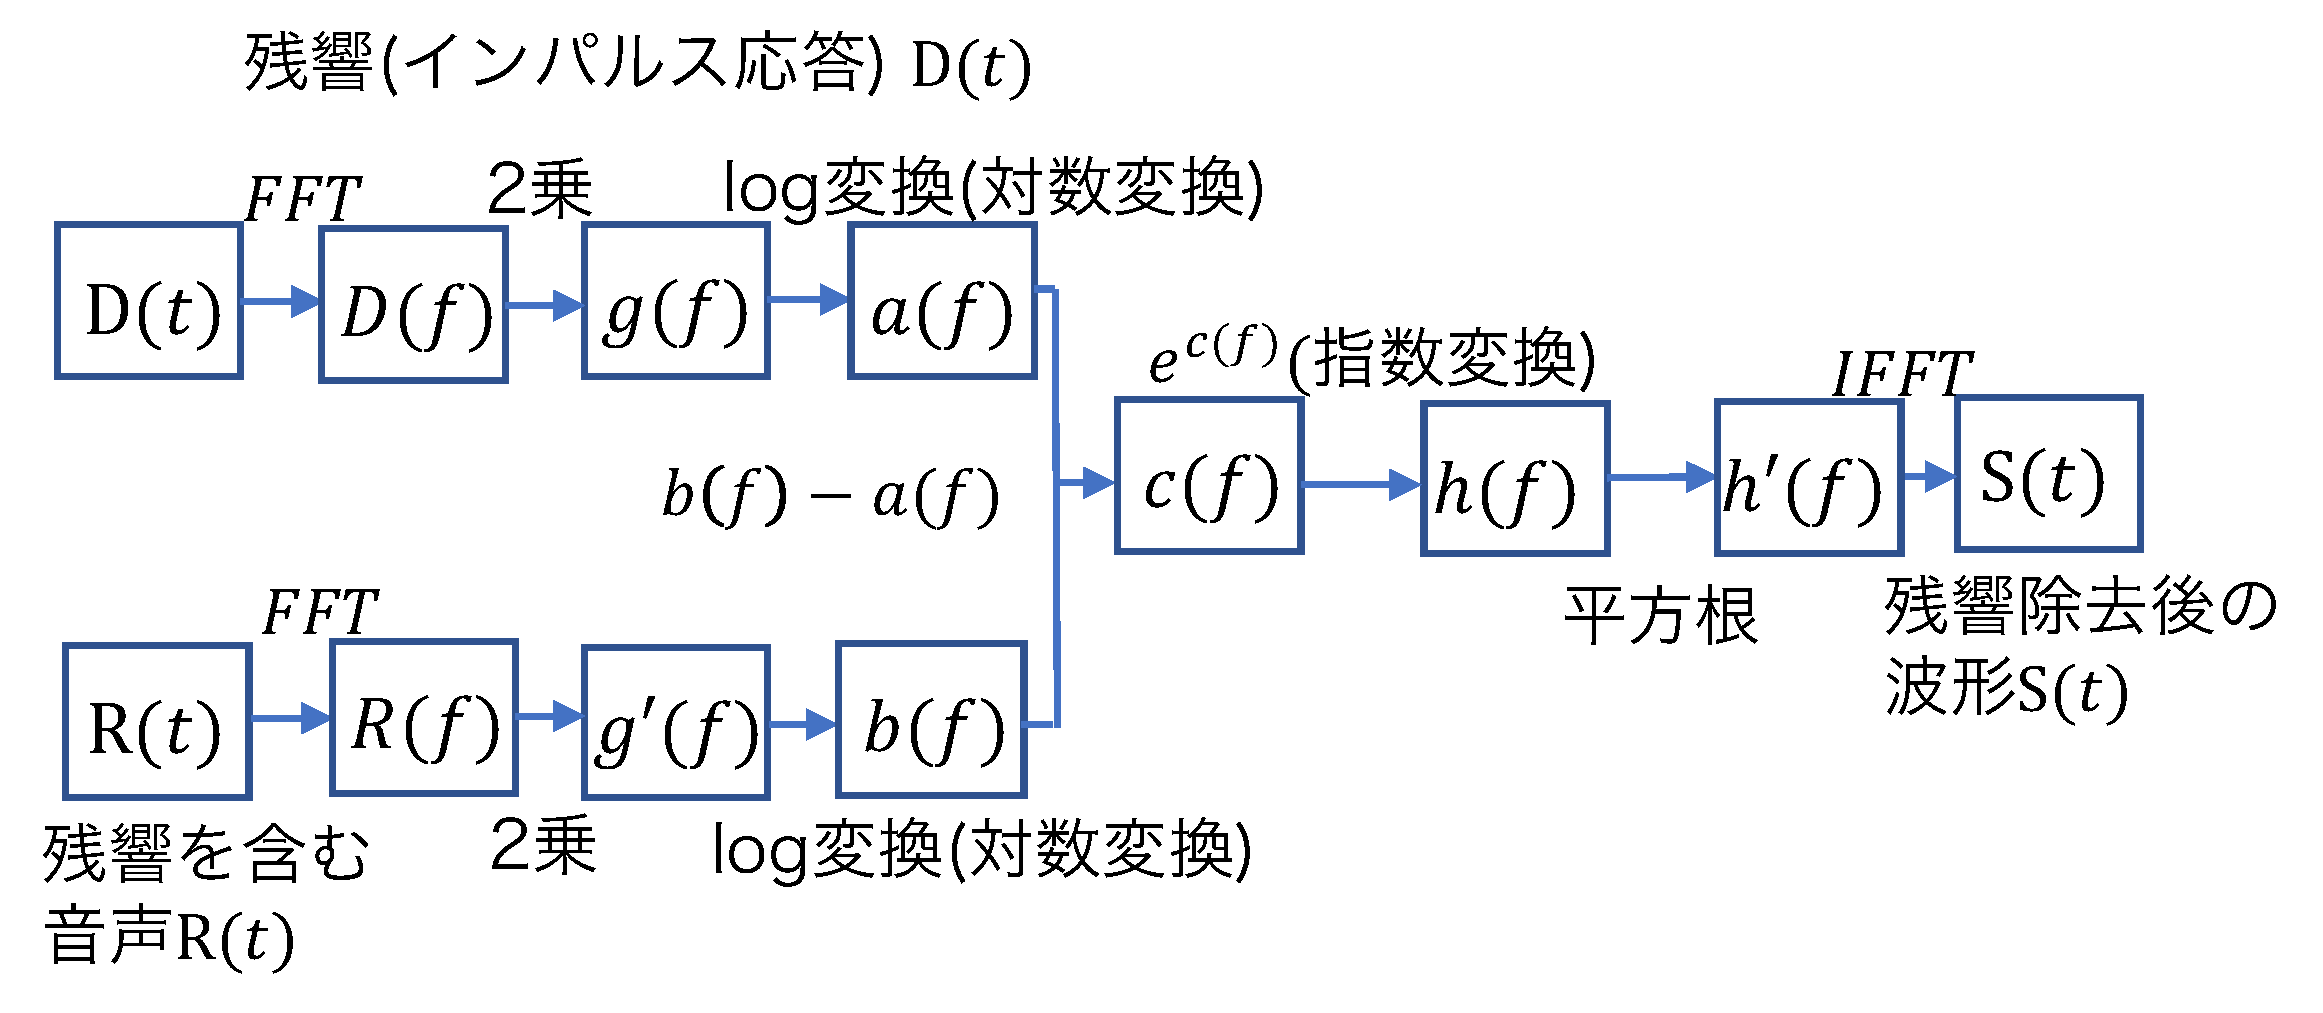
\includegraphics[clip,width=140mm,height=65mm]{riron.pdf}
\end{center}
 \caption{演算理論}
 \label{fig:cepst}
\end{figure}

D$(t)$,R$(t)$をFFTすることにより,$D(f)$と$R(f)$を求めることができる.$D(f)$と$R(f)$はともに周波数成分である.
{\Large
\begin{equation}
\label{提案手法最初}
  D(f) = \int^{\infty}_{-\infty}D(t)e^{(-j2\pi f)}dt 
\end{equation}
}

{\Large
\begin{equation}
\label{提案手法最初}
  R(f) = \int^{\infty}_{-\infty}R(t)e^{(-j2\pi f)}dt \\
\end{equation}
}

D$(f)$,R$(f)$を2乗することにより,$g(f)$と$g'(f)$を求めることができる.
{\Large
\begin{equation}
\label{提案手法最初}
  g(f) = |D(f)|^2
\end{equation}
}

{\Large
\begin{equation}
\label{提案手法最初}
  g'(f) = |R(f)|^2
\end{equation}
}

$g(f)$と$g'(f)$を対数変換することで$a(f)$と$b(f)$を求めることができる.対数処理をすることによって積商の計算に和差の計算に変換することができ,信号の分離を減法で行える.
{\Large
\begin{equation}
\label{提案手法最初}
  a(f) = \log g(f)
\end{equation}
}


{\Large
\begin{equation}
\label{提案手法最初}
  b(f) = \log g'(f)
\end{equation}
}
$b(f)-a(f)$することでR$(t)$に含まれるD$(t)$を取り除くことができ,元信号を抽出できると考えた.
{\Large
\begin{equation}
\label{提案手法最初}
  c(f) = b(f)-a(f)
\end{equation}
}
$b(f)-a(f)$により求めることができた$c(f)$を逆の工程を行うことで波形を時間領域に戻す.$c(f)$を対数変換により$h(f)$を求める.
{\Large
\begin{equation}
\label{提案手法最初}
  h(f) = e^{c(f)}
\end{equation}
}
$h(f)$の平方根を取ることによりにより$h'(f)$を求める.
{\Large
\begin{equation}
\label{提案手法最初}
  h'(f) =  \sqrt{h(f)}
\end{equation}
}

$h'(f)$をIFFTすることでS$(t)$を求めることで放送に内容と同等波形を取り出すことができると考えた.
{\Large
\begin{equation}
	\label{noref}
  S(t) =  \int^{\infty}_{-\infty}h'(f)e^{(j2\pi f)}dt 
\end{equation}
}


\newpage

\section{実験と検証}
\subsection{調査目的}
今回の実験の調査目的は本研究で研究した残響除去を行った場合,正しく聞き取れることができるかどうかである.よって,複数人に対して聴覚実験を行った.本研究の聴覚実験では,擬似的に残響を付与した音声波形と,その波形から残響音除去の処理を施した音声の波形を用いた.地震発生時を想定した際の避難を促す文章や,津波警報が発令時に避難を促す文章など6秒から18秒の音声を計4編用意した.この4編に対して,残響を擬似的に付加させた音声とその残響を除去した音声,計8編を実験に用いた.被験者には残響音付きの音声2編と除去後の音声2編の計4編を無作為に聞いたもらった.聞きながら文章を書き出してもらい,正答率を式(\ref{seitouritu})とした.
\begin{equation}
	\label{seitouritu}
  正答率 = \frac{聞き取れた文字数}{放送内容の文字数}
\end{equation}
放送内容を以下に示す.
\begin{itemize}
\item 緊急地震速報,強い揺れに警戒してください.\\
揺れが収まるまで安全を確保してください.
\item 津波警報が発令されました.\\
海岸付近の方は高台に避難してください.
\item こちらは防災センターです.\\
先程,火災感知器が作動しましたが,現場を確認した結果,誤報であることが確認できましたのでご安心ください.
\item 暴風警報が発令されました.\\
市内の皆様は,最寄りの避難所に避難してください.
\end{itemize}

\newpage
擬似的に付加させた残響を図\ref{fig:zatuon}に示す.今回使用したのは教会で録音されたインパルス応答と洞窟で録音されたインパルス応答を畳み込んだものになる.畳み込んだ理由として災害時に発生すると考えられる雑音は単体のインパルス応答で畳み込んだ場合より多く雑音が入ると考えた.そのため2つのインパルス応答を畳み込んだものを使用した.

\begin{figure}[h]
\begin{center}
 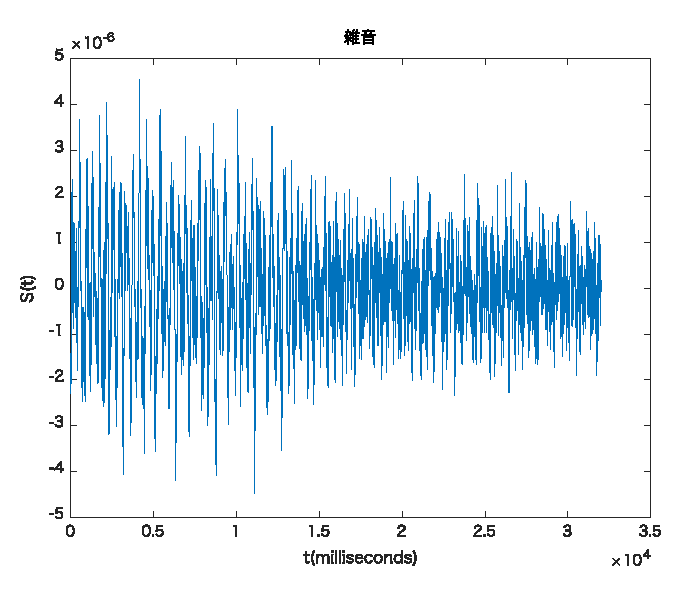
\includegraphics[clip,width=100mm,height=70mm]{zatsuon.pdf}
\end{center}
 \caption{付加させた残響}
 \label{fig:zatuon}
\end{figure}

\subsection{調査方法}
今回,実施した残響除去が有用であるかどうかを検証するために複数人に対し,聴覚実験の協力をしたもらった.

今回使用した実行環境を表\ref{tab:use}に示す.

\begin{table}[htb]
\begin{center}

\caption{実行環境}
  \begin{tabular}{|c|c|} \hline
    パソコン & iMac  \\ \hline
    OS & macOS  \\ \hline
    数値計算ソフトウェア & MATLAB\_R2019B  \\ \hline
    使用ヘッドホン & audio-technica ATH-ES10  \\ \hline
    実験協力人数 & 6名  \\ \hline
    音声サンプルレート & 44,100Hz  \\ \hline
    ビット/サンプル & 16ビット/サンプル  \\ \hline
    チャンネル数 & モノラル  \\ \hline
    実験場所 & 津田沼校舎,7号館7階第12研究室\\ \hline
  \end{tabular}
  \label{tab:use}
  \end{center}
\end{table}

\newpage

\subsection{回答の集計と効果の検証}
今回の実験結果,文章の正答率を図(\ref{fig:shitsumonshi}),回答例を図(\ref{fig:kaitourei1}),(\ref{fig:kaitourei2})に示す.



\begin{figure}[h]
\begin{center}
 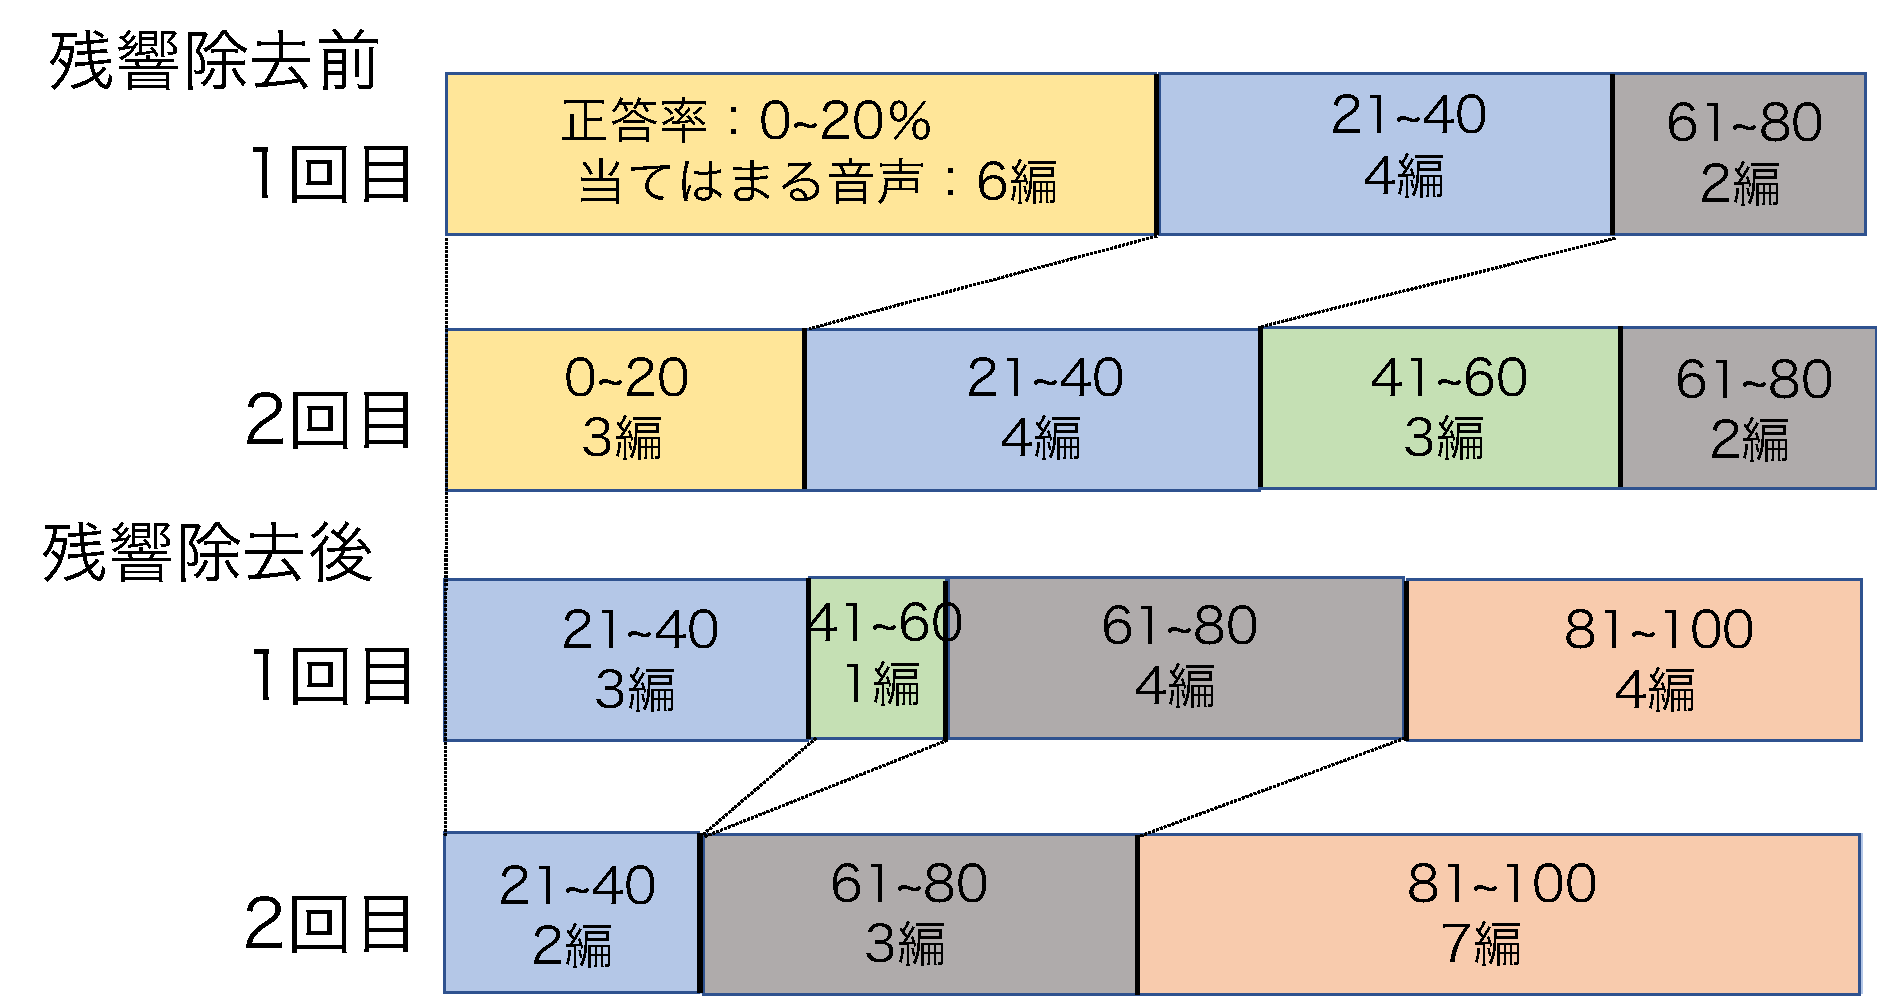
\includegraphics[clip,width=130mm,height=80mm]{shitsumonkekka.pdf}
\end{center}
 \caption{実験結果}
 \label{fig:shitsumonshi}
\end{figure}
 
残響が付加されている音声が上2つ,残響が除去された音声が下2つになっている.

残響除去前の1回目と2回目を比べる.正答率0	\textasciitilde20\%が6編から3編に減少している.正答率21\textasciitilde40\%が4編から4編と変化はない.正答率41\textasciitilde60\%が0編から3編と増加している.正答率61\textasciitilde80\%が2編から2編と変化はない.残響前の音声でも2回聞くことにより,聞き取りやすさが上昇していることがわかる.しかし,全体的に見ても聞き取りやすさの上昇は少ないといえる.

残響除去後の1回目と2回目を比べる.正答率0	\textasciitilde20\%が0編から0編は変化はない.正答率21\textasciitilde40\%が3編から2編と減少している.正答率41\textasciitilde60\%が1編から0編と減少している.正答率61\textasciitilde80\%が4編から3編と減少している.正答率81\textasciitilde100\%が4編から7編と増加している.残響後の音声は2回聞くことにより,聞き取りやすさが上昇し,8割の音声が60\%以上聞き取ることができていることがわかる.しかし,全体的な聞き取りやすさの上昇は少ないといえる.

残響除去前の1回目と除去後の1回目を比べる.正答率0	\textasciitilde20\%が除去前は6編であり,12編の中で一番多いのに対し,除去後は1編もない.正答率21\textasciitilde40\%,除去前が4編なのに対し除去後は3編,正答率41\textasciitilde60\%が除去前が0編なのに対し除去後が1編,正答率61\textasciitilde80\%が除去前2編なのに対し除去後が4編とあまり変わらないのがわかる.しかし,正答率81\textasciitilde100\%になると除去前0編なのに対し除去後4編と.除去後は$1/3$の音声がほとんど聞き取れていることがわかる.

残響除去前の2回目と除去後の2回目を比べる.正答率0	\textasciitilde20\%が除去前は3編であり,除去後は1編もない.正答率21\textasciitilde40\%,除去前が4編なのに対し除去後は2編,正答率41\textasciitilde60\%が除去前が3編なのに対し除去後が0編,正答率61\textasciitilde80\%が除去前2編なのに対し除去後が3編とあまり変わらないのがわかる.やはり,正答率81\textasciitilde100\%になると除去前0編なのに対し除去後7編と,音声を1回目聞いたときの比較より大きく開いている.

このことからも除去前後関わらず音声を2回聞くことにより正答率は上がることがわかる.また,除去前後で比べると前は41\%以上聞き取れているものが2回聞いても半分に達しなかったが,除去後は1回目の時点から41\%以上が$3/4$を締めていることがわかる.


\begin{comment}
 除去前の音声では1回目では6編(50\%)の音声の正答率が0	\textasciitilde20\%になっていることからも聞き取りづらいことがよく分かる.
また,2回聞いて61\%以上聞き取れているものが2編(20\%)だったのに対し,
除去後の音声では1回しか聞いていないにもかかわらず61\%以上聞き取れている音声が8編(70\%)あることからも聞き取りやすくなっていることがわかる.

加えて行った放送内容が理解できたかという問いに対しても残響を付加している音声より除去後の音声のほうが内容を理解して聞き取れていることがわかる.
\end{comment}

% \newpage
 
\begin{figure}[h]
\begin{center}
 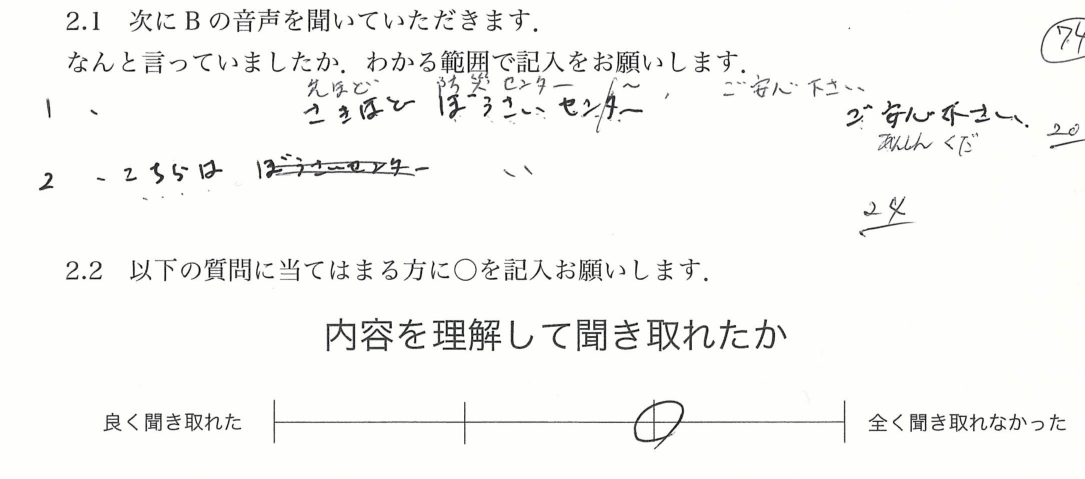
\includegraphics[clip,width=130mm,height=55mm]{kaitourei1.pdf}
\end{center}
 \caption{回答例1(残響除去前)}
 \label{fig:kaitourei1}
\end{figure}

\begin{figure}[h]
\begin{center}
 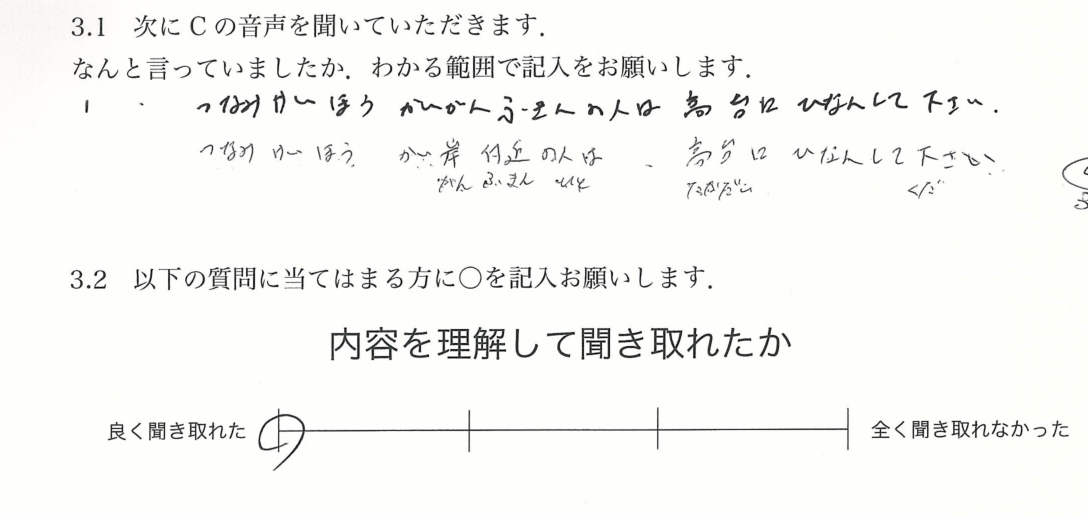
\includegraphics[clip,width=130mm,height=55mm]{kaitourei2.pdf}
\end{center}
 \caption{回答例2(残響音除去後)}
 \label{fig:kaitourei2}
\end{figure}

\newpage

\subsection{考察}
逆畳込みとケプストラム法を組み合わせた音声による聴覚実験において,残響除去は成功し,放送内容を聞き取りやすくなったと考えられる.また,今回の実験では6名と比較的に少数による実験であったが,もっと多くの人数と多くの音声サンプルを用いれば,よりはっきりとした違いが現れるだろう.

しかし,今回の実験,検証において残響音を擬似的に畳み込んだものを使用している.実際の行政放送では残響音だけでなく,外部からの音による聞き取りづらさ,地形的な放送機同士の干渉など考えなければいけないことはまだ多い.また,質問用紙の「このような反射の含まれた(または含まれていない)非常放送は聞き覚えがあるか」という問いは,残響による聞き取りづらさを経験の有無を問う主旨で設問された.しかし,放送内容に聞き覚えがあるかという残響経験の確認ではなく,文章内容自体の確認になってしまっていたことがあった.そのため,質問の文章をより考えなければいけない
.

\newpage
\section{結言}
日本は他国よりも災害が多い.そのため,町内放送などの非常放送の重要性がとても高い\cite{oka1}.屋外やデパートなどの屋内,トンネルの中など様々な場所で,館内放送や非常放送の整備されている.しかし,スピーカから離れている地点で放送を聞くと建物などによる反射音により,内容を聞き取りづらいことが多い.
%ここで,信号処理によって反射音を除去できれば,放送内容を聞き取ることが可能となる.
また,火災が発生した場合,屋内のスピーカからの非常放送を屋内で受聴することになるが,反射や残響によって聞き取りづらいことが懸念される.


そのため,残響を除去させる方法として佐藤の研究では非常放送の音声の先頭に信号音を付加させた\cite{oka2}.その信号を基準としてディジタルデバイスによってリアルタイムにインパルス応答を計算し,余分な残響を除去する方法を提案した.しかし,実際の音声を用いて検証したところ,うまく動作しなかった.

%目的
そこで本研究では,逆畳込みとケプストラム法を組み合わせることにより,非常放送を明瞭に聞き取るための手法を考察し,検証を目的とした.結果として,残響を除去でき,明瞭度を図る実験において聞き取りやすくなったという回答が多かった.しかし,本研究では実環境で録音したものではなく残響を擬似的に付加させたものを使用した.実際に放送を聞く環境においてはより多くの聞き取りづらくなる要因が考えられる.今後,本研究の結果をもとに実環境での実験が望まれる.

\newpage
\section*{謝辞}
\addcontentsline{toc}{section}{謝辞}
本研究の遂行および本論文の作成にあたり,多くの御助言と御指導をいただきました須田宇宙准教授に深く感謝の意を表します.
本研究の遂行および本論文の作成にあたり,多くの御助言と御指導をいただきました大川研究室の坂口智弘先輩に深く感謝の意を表します.

\newpage
\bibliographystyle{jplain}
\addcontentsline{toc}{section}{参考文献}
\begin{thebibliography}{99}

\bibitem{oka1}国土技術センター,``自然災害の多い国'',
http://www.jice.or.jp/knowledge/japan/commentary09
\bibitem{oka2}佐藤 由希子,``インパルス応答を用いた反射音除去のための一提案'', 千葉工業大学卒業論文, 2014
\bibitem{oka3}小泉 宣夫,``基礎音響・オーディオ学'',コロナ社 ,2005
\bibitem{oka4}青木 直史,``デジタル・サラウンド処理入門'',CQ出版,2006
\bibitem{oka5}日本音響学会編,``音響学入門ペディア'',コロナ社,2017
\bibitem{oka6}小野測器,``FFT解析に関する基礎用語集'',
\url{https://www.onosokki.co.jp/HP-WK/c_support/tech_term/cf_fft/cf3.htm}
\bibitem{oka7}総務省,``平成23年(2011年)東北地方太平洋沖地震(東日本大震災)の被害状況(平成30年3月1日現在)''
\url{ttps://www.soumu.go.jp/menu_news/s-news/01shoubo01_02000025.html}
\end{thebibliography}

\newpage
\section*{付録}
\addcontentsline{toc}{section}{付録}
\appendix
\section{ソースコード}


\begin{lstlisting}[caption=残響除去,label=fuga]
format long g;

 Fs=44100;        %Sampling frequency

[FileName, PathName] = uigetfile('*.wav', 'インパルス応答を選択');

T = strcat(PathName, FileName);
[data1,Fs1] = audioread(T);%データの読み込み

[FileName, PathName] = uigetfile('*.wav', '元になる音を選択');

T = strcat(PathName, FileName);

[data2,Fs2] = audioread(T);%データの読み込み

[FileName, PathName] = uigetfile('*.wav', '元になる音を選択');

T = strcat(PathName, FileName);

[data3,Fs3] = audioread(T);%データの読み込み

%% 元波形作成

signal = data2+1;


figure();
plot(signal)
title('元波形')


%% 元波形にインパルス応答畳み込み(反射音を含む音声の作成)

ref = data1;
ref = conv(ref,data3,'same');
figure();
plot(ref)
title('ImpulseResponse')

 refsignal = conv(signal,ref,'full');
 
 figure();
 plot(refsignal)
 title('反射音を含んだ波形')
 
 figure();
 plot(ref)
 title('反射音')


%% 逆畳み込みによりインパルス応答の抽出

[q,r] = deconv(refsignal,signal);

figure();
plot(q)%反射音の削除された音声 逆畳み込みによって求められた商
title('Impulse Response q 逆畳み込みによって求められた商')

figure();
plot(r)%逆畳み込みによって求められた剰余
title('No refrection Signal Voice r 逆畳み込みによって求められた剰余')
xlabel('t(milliseconds)')
ylabel('S(t)')


%% 波形の長さ揃える

len_sig = length(signal);
len_refsig = length(refsignal);
len_diff = len_refsig - len_sig;
add = zeros(len_diff,1);
signal = vertcat(signal,add);

%% ケプストラム法

signal1 = fft(signal);
signal1 = (signal1.*signal1);
signal1 = log(signal1);

refsignal1 =fft(refsignal);
refsignal1 = (refsignal1.*refsignal1);
refsignal1 = log(refsignal1);

figure();
plot(signal1)
plot(abs(signal1))
title('signal1')
figure();
plot(abs(refsignal1))
title('refsignal1')

len_q = length(q);
len_diffs = len_refsig - len_q;
addf = zeros(len_diffs,1);
q1 = vertcat(q,addf);
figure();
plot(abs(q1))
title('ref1')

q1 = fft(q1);
q1 = (q1.*q1);
q1 = log(q1);
figure();
plot(abs(q1))
title('ref1')

kep = refsignal1 - q1;
figure();
plot(kep)
plot(abs(kep))
title('kep')

norefsiga = refsignal1 - q1;
norefsiga1 = norefsiga - log(fft(signal));
norefsiga2 = exp(norefsiga1);
norefsiga2 = ifft(norefsiga2);

figure();
plot(norefsiga2)
title('パターンA absなし')

figure();
plot(abs(norefsiga2(1:622088)))
title('パターンA absあり')


%% ファイルとして保存

refsignals =refsignal./max(refsignal);
norefsigas = norefsiga2./max(norefsiga2);


audiowrite('残響付き波形名前.wav',refsignals,Fs2,'BitsPerSample',16);

audiowrite('残響除去波形名前.wav',norefsigas,Fs2,'BitsPerSample',16)

\end{lstlisting}
\newpage
\section{質問用紙}
\begin{figure}[h]
\begin{center}
 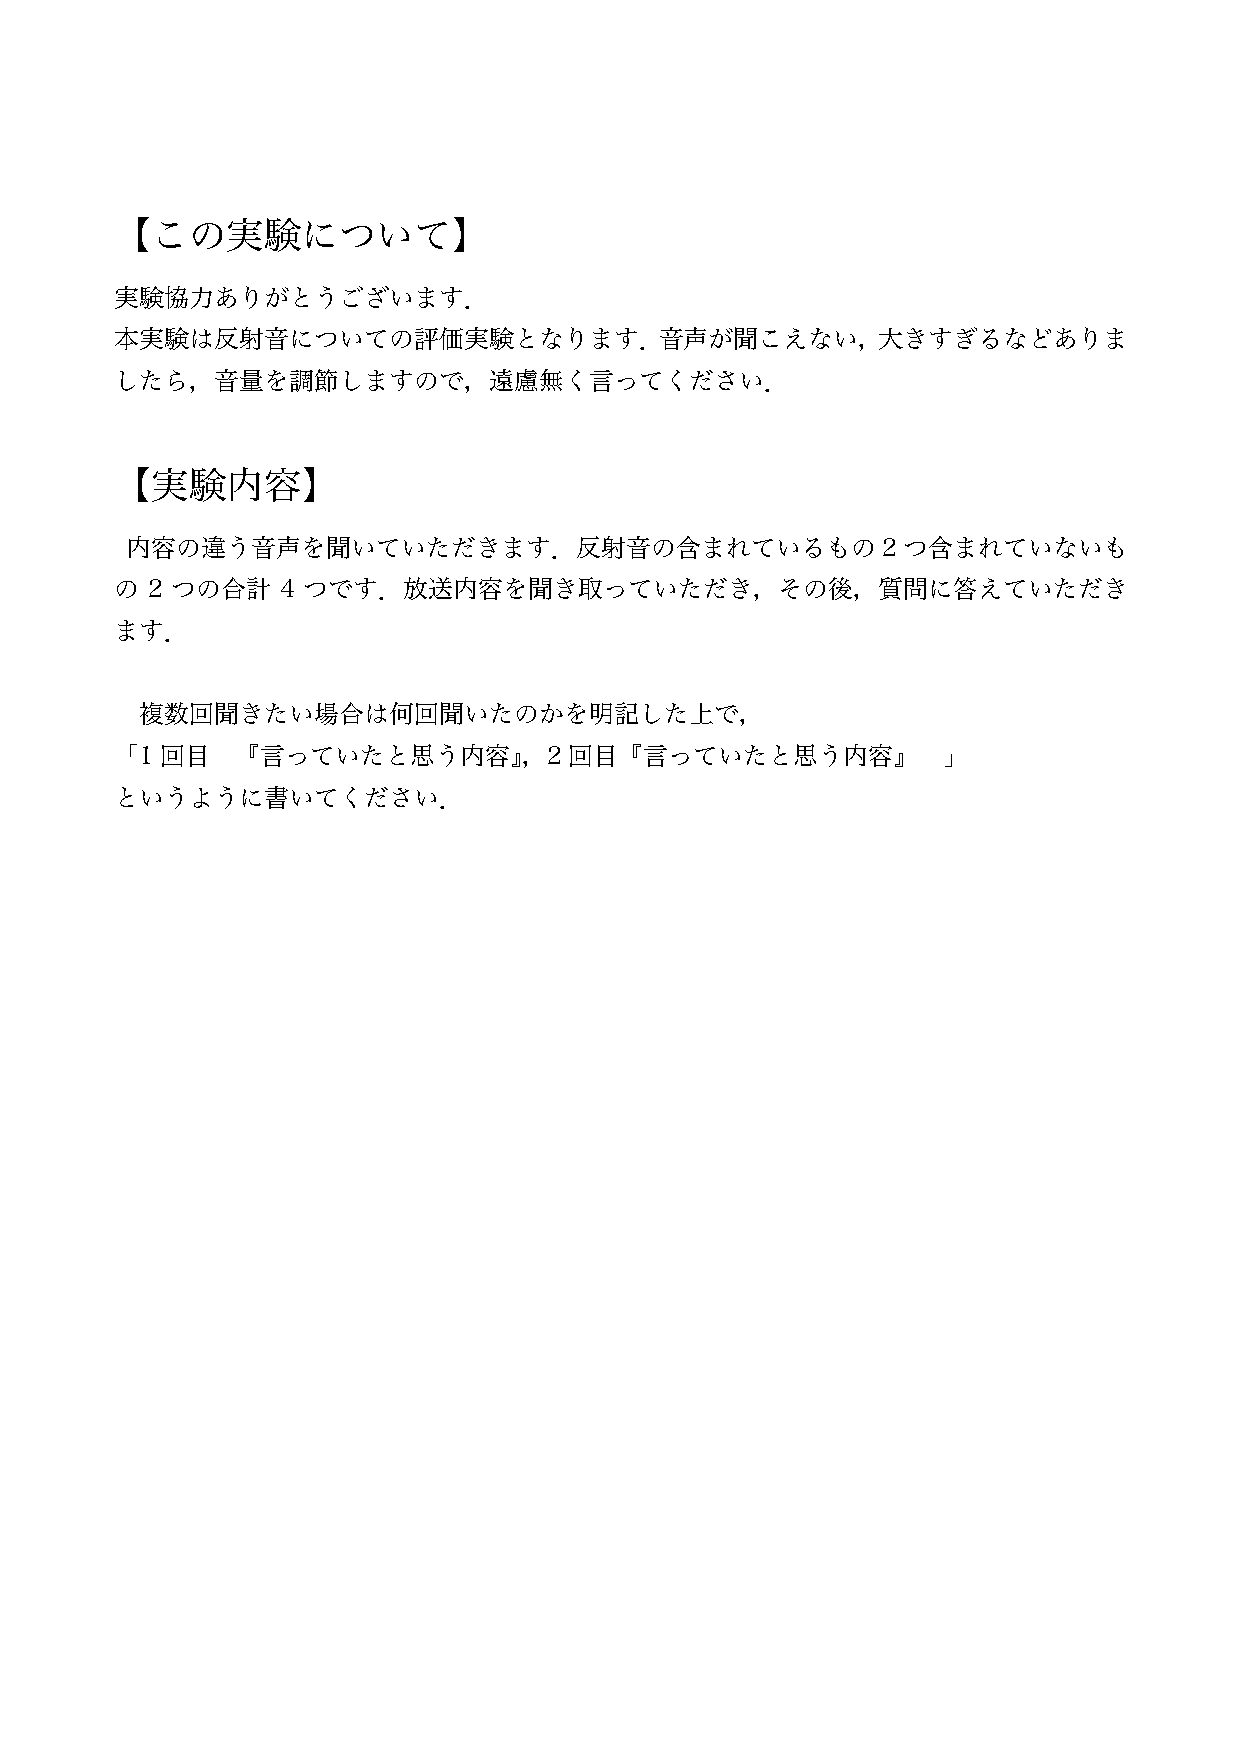
\includegraphics[clip,width=180mm,height=240mm]{shitsumonshi1.pdf}
\end{center}
 \label{fig:kaitourei2}
\end{figure}
\begin{figure}[h]
\begin{center}
 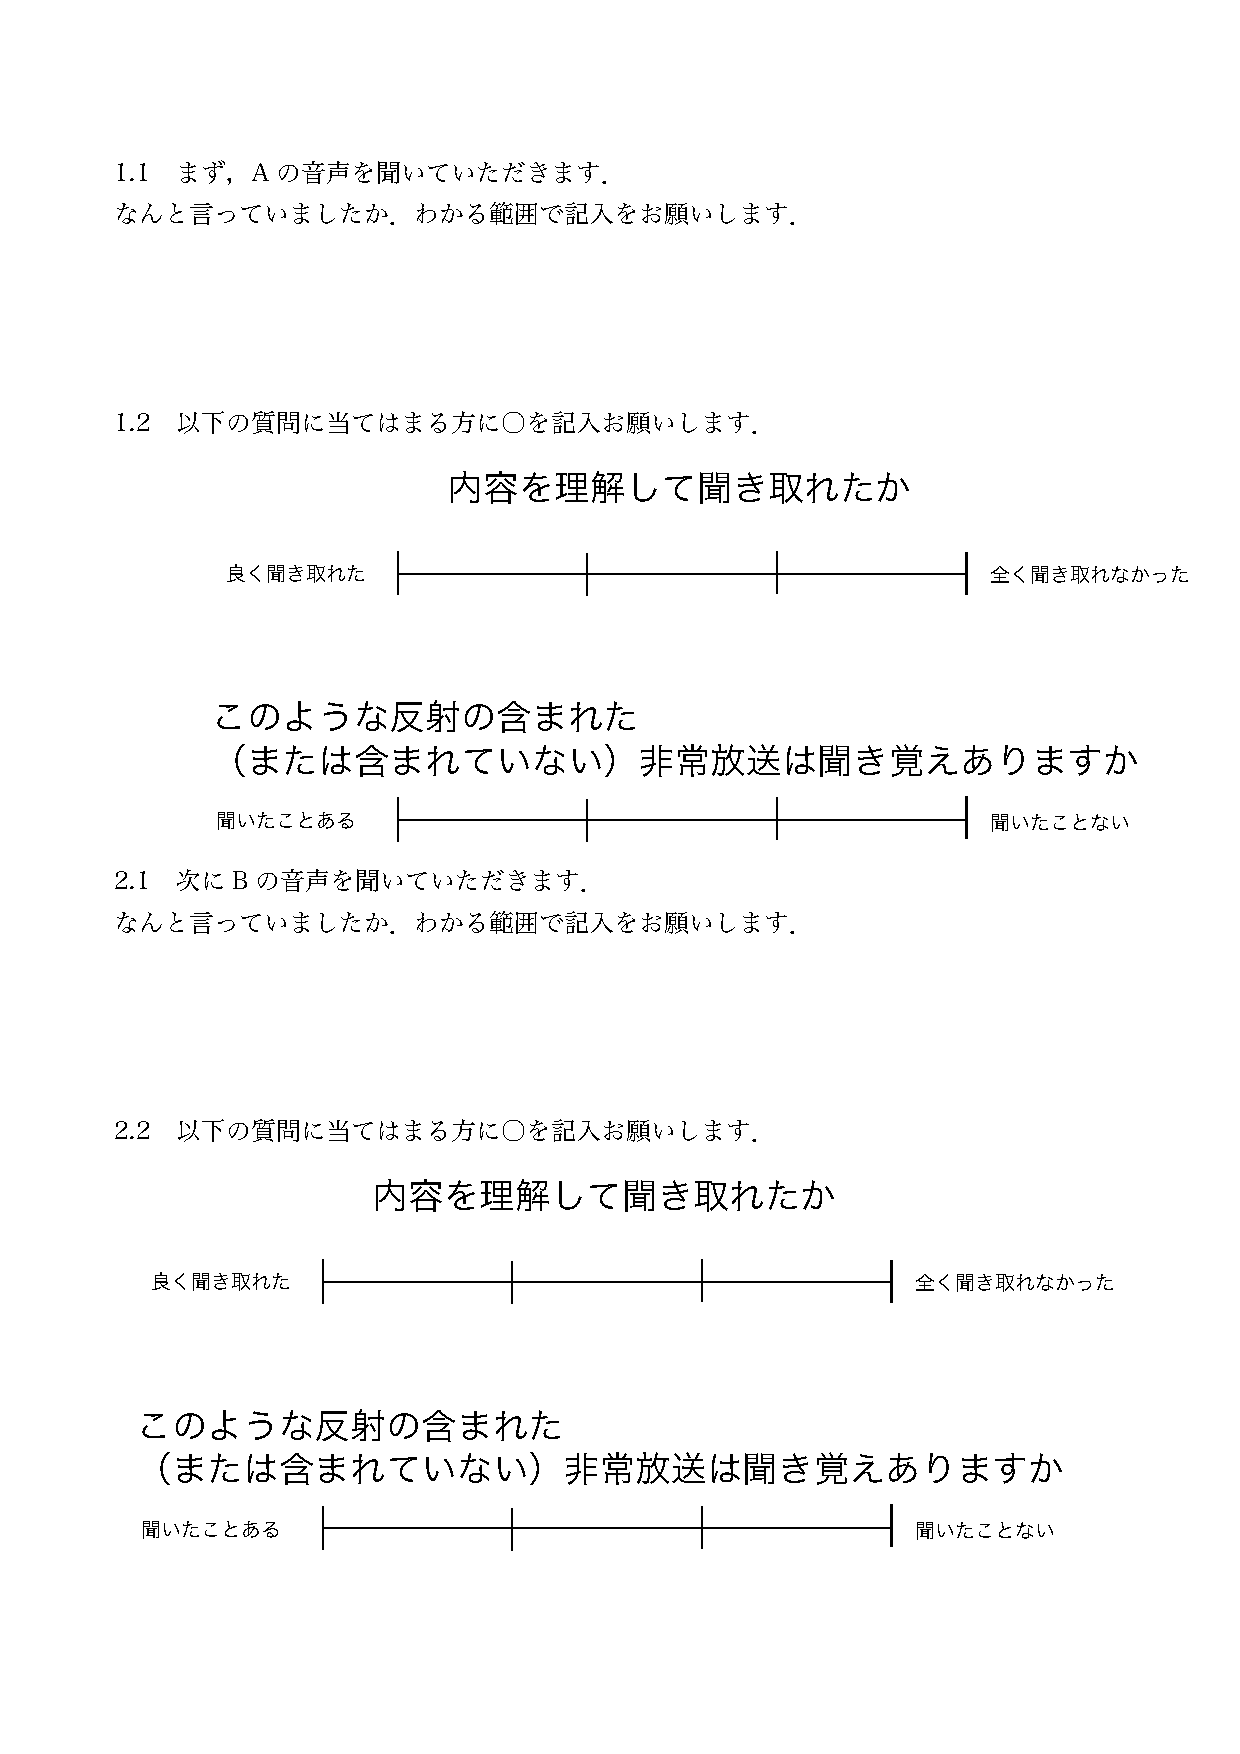
\includegraphics[clip,width=180mm,height=240mm]{shitsumonshi2.pdf}
\end{center}
 \label{fig:kaitourei2}
\end{figure}
\begin{figure}[h]
\begin{center}
 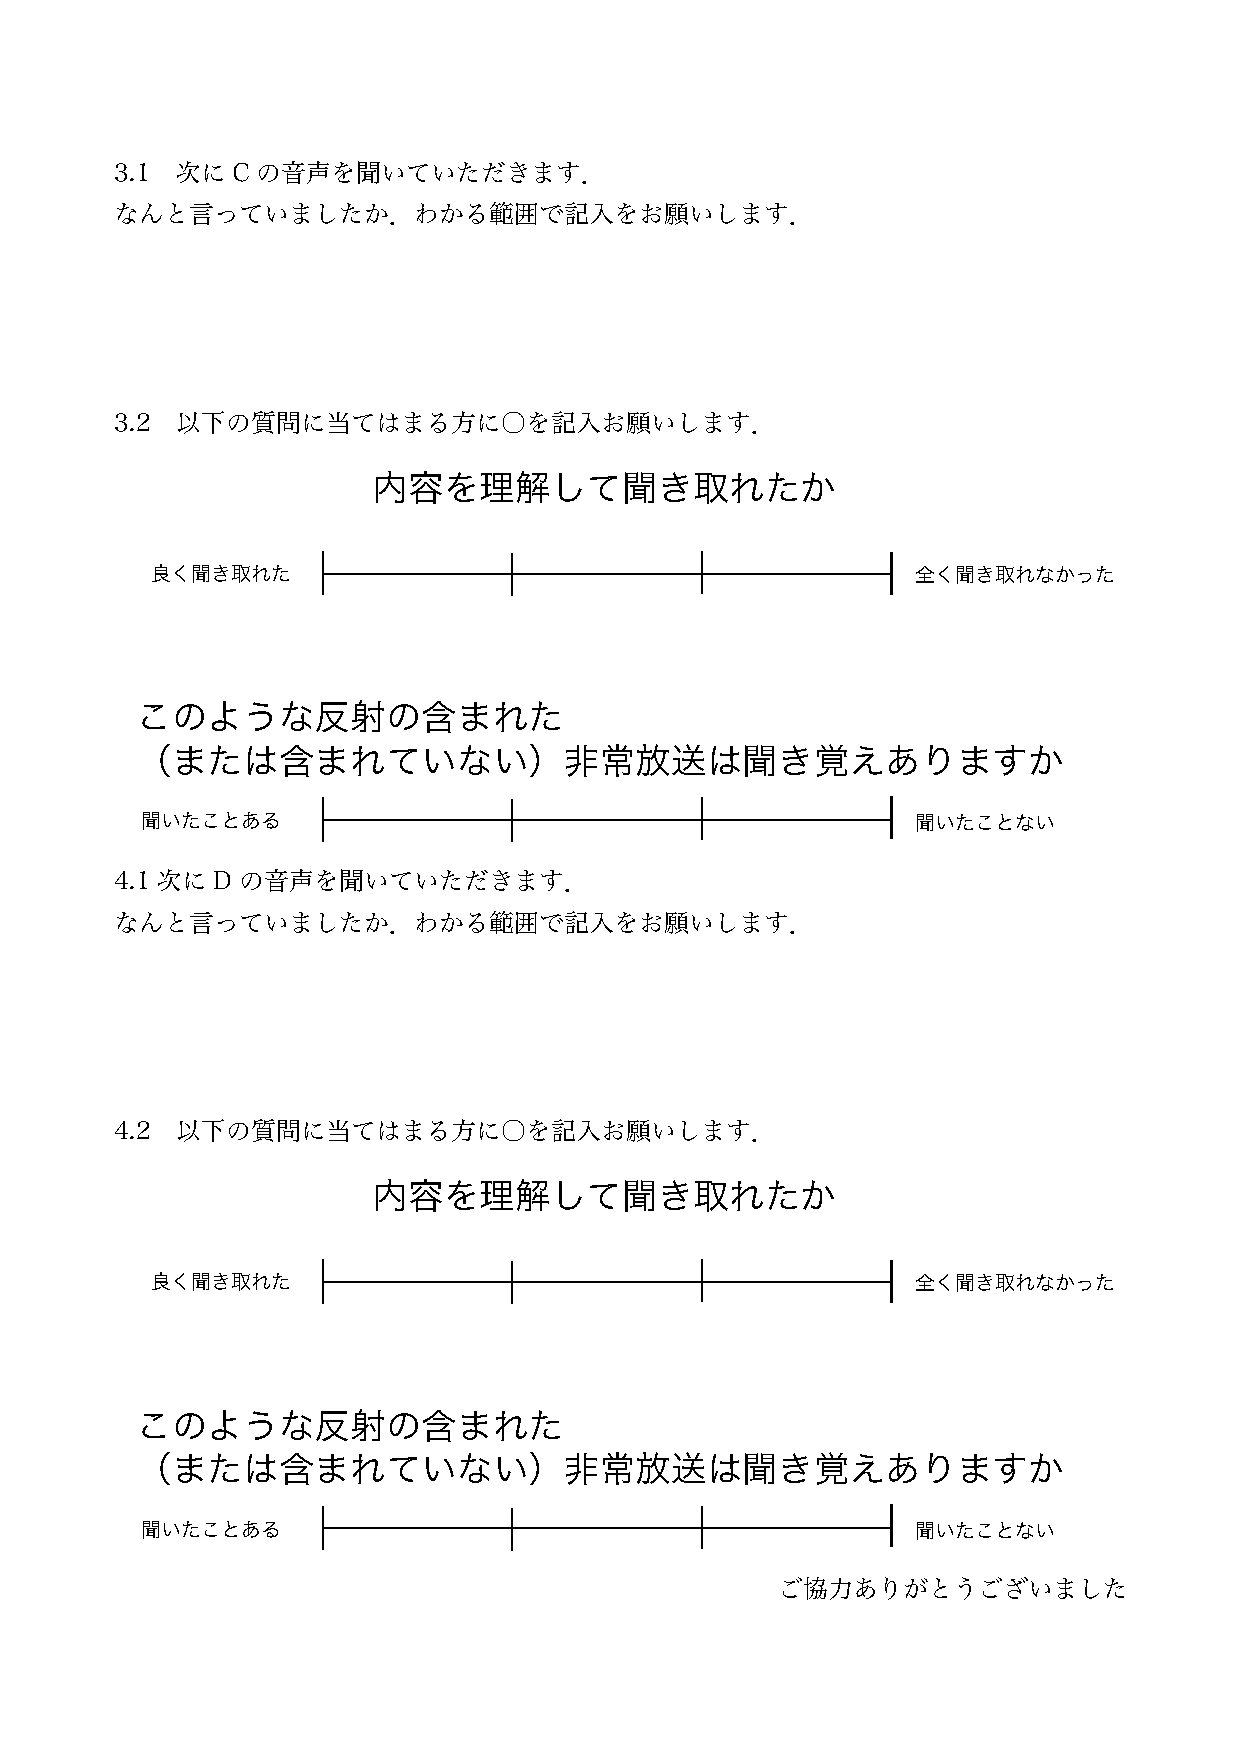
\includegraphics[clip,width=180mm,height=240mm]{shitsumonshi3.pdf}
\end{center}
 \label{fig:kaitourei2}
\end{figure}


\end{document}
